% UUM 523E Ara Proje raporu (Türkçe), Grup 2
% Overleaf'te AIAA şablonunun new-aiaa.cls sınıfıyla derlenir; new-aiaa.cls bu dosyayla
% aynı klasörde olmalıdır. tables/*.tex dosyaları MT_Group2.mat ve HW2_Group2.mat değerlerini içerir.
\documentclass[conf]{new-aiaa}
\usepackage[T1]{fontenc}
\usepackage[utf8]{inputenc}
\usepackage[turkish,shorthands=off]{babel}
\usepackage{icomma}
\usepackage{graphicx}
\usepackage{amsmath}
\usepackage{booktabs}
\usepackage{multirow}
\usepackage{longtable,tabularx}
\setlength\LTleft{0pt}
% Tablo gövdeleri ilkel \@@input ile okunur: LaTeX'in \input komutu genişletilemez
% olduğundan tablo içinde ardından gelen \bottomrule "Misplaced \noalign" hatası verir.
\makeatletter
\newcommand\tabinput[1]{\@@input #1 }
\makeatother
\makeatletter
\AtBeginDocument{\@ifpackageloaded{hyperref}{\hypersetup{hidelinks}}{}}  % bağlantı çerçeveleri gizli
\makeatother
\AtBeginDocument{%
  \renewcommand\figurename{Şekil}%
  \renewcommand\tablename{Tablo}%
  \renewcommand\refname{Kaynaklar}}

\title{F-16 Uçak Modeli, Trim, Trim Uçuşu Benzetimi ve Kararlılık Analizi}

\author{Dilan Gelturan, Emirhan Oskay, Emircan Sürücü ve Berat Alku\footnote{Yüksek lisans öğrencileri, Uçak ve Uzay Bilimleri Fakültesi; UUM 523E İleri Uçuş Dinamiği, Grup 2.}}
\affil{İstanbul Teknik Üniversitesi, 34469 Maslak, İstanbul, Türkiye}

\begin{document}

\maketitle

\begin{abstract}
NASA TP-1538 aerodinamik ve motor verilerinden Simulink'te altı serbestlik dereceli, doğrusal olmayan bir F-16 modeli kurulmuş, kısıtlı bir eniyileme yöntemiyle trimlenmiş ve gövde ile rüzgâr eksenlerinde sayısal olarak doğrusallaştırılmıştır. Bu raporda bu çalışma özetlenmekte ve 0,6 Mach ile 10\,000 ft'te üç trim koşulu incelenmektedir: ağırlık merkezi $0,25\bar c$'de kanatlar düz uçuş (i), $60^\circ$ yatışlı düz dönüş (ii) ve ağırlık merkezi $0,35\bar c$'de kanatlar düz uçuş (iii). Trim noktalarından kumandalar sabit tutularak başlatılan doğrusal olmayan model, i ve ii koşullarında 60~s boyunca ve bir tam dönüş süresince trimi korumaktadır; sapmalar $10^{-2}$~m/s ve $10^{-3}$ derecenin altındadır. iii koşulunda ise durumlar yavaşça ıraksamaktadır. Kararlılık parametreleri ve boyutsuz türevler rüzgâr ekseni durum matrislerinden çıkarılmış; yuvarlanma ve sapma satırlarındaki eylemsizlik bağlaşımı ayrıştırılmış, itkinin hız sönümüne katkısı motor modelinden hesaplanmıştır. iii koşulunda uçak boyuna eksende statik olarak kararsızdır ($C_{m_\alpha}=+0,156$~rad$^{-1}$) ve kısa periyot modu iki gerçel köke ayrılır; bunlardan biri için genliğin iki katına çıkma süresi 0,88~s'dir. Dönüşte trim açısal hızları durum matrisine eylemsizlik terimleri ekler ve fugoid ile spiral modlarını birbirine bağlar; bu bağlaşım fugoid periyodunu 120~s'den 57~s'ye kısaltır.
\end{abstract}

\section*{Semboller}

{\renewcommand\arraystretch{1.0}
\noindent\begin{longtable*}{@{}l @{\quad=\quad} l@{}}
$A$, $B$ & doğrusal modelin durum ve giriş matrisleri \\
$a_{ij}$ & $A$'nın $(i,j)$ elemanı \\
$b$, $\bar c$, $S$ & kanat açıklığı, ortalama aerodinamik veter, kanat alanı; m, m, m$^2$ \\
$C_D$, $C_L$ & sürükleme ve kaldırma katsayıları \\
$C_l$, $C_m$, $C_n$ & yuvarlanma, yunuslama ve sapma momenti katsayıları \\
$C_{D_u}$, $C_{m_u}$ & $\Delta V_T/U_1$'e göre türevler \\
$C_{(\cdot)_\alpha}$, $C_{(\cdot)_\beta}$ & $\alpha$ ve $\beta$'ya göre türevler, rad$^{-1}$ \\
$C_{(\cdot)_q}$ & $q\bar c/(2U_1)$'e göre türev, rad$^{-1}$ \\
$C_{(\cdot)_p}$, $C_{(\cdot)_r}$ & $pb/(2U_1)$ ve $rb/(2U_1)$'e göre türevler, rad$^{-1}$ \\
$h$ & irtifa, m \\
$h_E$ & motorun açısal momentumu, kg\,m$^2$/s \\
$I_{xx}$, $I_{yy}$, $I_{zz}$, $I_{xz}$ & eylemsizlik momentleri ve çarpımı (gövde ekseni), kg\,m$^2$ \\
$L_{(\cdot)}$, $M_{(\cdot)}$, $N_{(\cdot)}$ & yuvarlanma, yunuslama ve sapma kararlılık parametreleri \\
$m$ & uçak kütlesi, kg \\
$n_z$ & normal yük faktörü \\
$p$, $q$, $r$ & gövde ekseni yuvarlanma, yunuslama ve sapma hızları, rad/s \\
$\bar q$ & dinamik basınç, Pa \\
$T$ & itki, N \\
$t_{1/2}$, $t_2$ & genliğin yarıya inme ve iki katına çıkma süreleri, s \\
$U_1$ & trimdeki toplam hız, m/s \\
$u$, $v$, $w$ & gövde ekseni hız bileşenleri, m/s \\
$V_T$ & toplam hız, m/s \\
$X_u$, $X_{T_u}$ & aerodinamik ve itki kaynaklı hız sönümü parametreleri, s$^{-1}$ \\
$x_N$, $y_E$ & kuzey ve doğu konumları, m \\
$x_{cg}$ & ağırlık merkezinin konumu, $\bar c$ cinsinden \\
$\alpha$, $\beta$ & hücum açısı ve yan kayma açısı, rad \\
$\gamma$ & uçuş yolu açısı, rad \\
$\delta_T$ & gaz kolu konumu, \% \\
$\delta_h$, $\delta_a$, $\delta_r$, $\delta_{lef}$ & stabilatör, kanatçık, dümen ve hücum kenarı flapı (LEF) açıları, rad \\
$\zeta$, $\omega_n$ & sönüm oranı, doğal frekans (rad/s) \\
$\lambda$ & özdeğer, s$^{-1}$ \\
$\tau$ & zaman sabiti, s \\
$\phi$, $\theta$, $\psi$ & yatış, yunuslama ve yön açıları, rad \\
$\boldsymbol\omega$ & gövde açısal hız vektörü $[p\ q\ r]^T$, rad/s \\
\multicolumn{2}{@{}l}{\emph{Alt indisler}}\\
$1$ & trim (kararlı hâl) değeri \\
$T$ & itki katkısı \\
\end{longtable*}}

\section{Giriş}

\lettrine{B}{u} rapor, UUM 523E dersinin dönem projesini üç adımda sunmaktadır. Ödev~1'de NASA TP-1538'in~\cite{tp1538} aerodinamik ve motor verileri, Stevens, Lewis ve Johnson'ın~\cite{slj} atmosfer modeli ve hareket denklemleriyle Simulink'te altı serbestlik dereceli, doğrusal olmayan bir F-16 modeli kurulmuştur. Ödev~2'de model altı uçuş koşulunda trimlenmiş ve bunların üçünde doğrusallaştırılmıştır. Ara Proje bu sonuçları, hepsi 0,6 Mach, 10\,000~ft ve $\gamma=0$ olan üç trim koşulunda kullanır:
\begin{enumerate}
\item[i.] kanatlar düz uçuş, $x_{cg}=0,25\bar c$;
\item[ii.] $\phi=60^\circ$ ve $\beta=0$ ile kararlı düz dönüş, $x_{cg}=0,25\bar c$;
\item[iii.] kanatlar düz uçuş, $x_{cg}=0,35\bar c$.
\end{enumerate}
Önce doğrusal olmayan model her trim noktasından kumandalar sabitken uçurulmuştur (Bölüm~IV). Ardından kararlılık parametreleri ve boyutsuz türevler rüzgâr ekseni durum matrislerinden çıkarılmış (Bölüm~V), dinamik modlar tam ve ayrık matrislerden hesaplanmıştır (Bölüm~VI). Bölüm~II ve III, bu analizlerin dayandığı uçak modelini ve trim ile doğrusallaştırma çalışmasını özetler.

Bütün analizler, Ödev~1'in modelini (\texttt{F16\_6DOF.slx}, R2023a'da kaydedilmiş; Ödev~1 geri bildirimine göre Bölüm~II.C'de anlatıldığı gibi düzeltilmiş) çağıran MATLAB m-dosyalarıyla yapılmıştır: \texttt{run\_HW1.m}, \texttt{run\_HW2.m} ve sonuç dosyası \texttt{MT\_Group2.mat}'ı yazan \texttt{run\_MT.m}. Bütün büyüklükler SI birimlerindedir; aksi belirtilmedikçe açılar radyandır.

\section{Uçak Modeli}

\subsection{Yapı}
Model (Şekil~\ref{fig:model}), Aerospace Blockset kullanılmadan temel Simulink bloklarıyla kurulmuş altı alt sistemden oluşur: Atmosfer, Aerodinamik, İtki, Kütle ve Eylemsizlik, Eyleyiciler ve Hareket Denklemleri. Hücum kenarı flapı (LEF) tarifesi kök seviyededir; Aerodinamik, İtki ile Kütle ve Eylemsizlik alt sistemleri kendi gövde ekseni kuvvet ve momentlerini verir, bunlar Hareket Denklemleri alt sisteminde toplanır. Kütle, eylemsizlik ve geometri TP-1538 Tablo~I'deki~\cite{tp1538} değerlerin SI karşılıklarıdır: $m=9298,64$~kg, $S=27,871$~m$^2$, $b=9,144$~m, $\bar c=3,4503$~m, $I_{xx}=12\,875$, $I_{yy}=75\,674$, $I_{zz}=85\,552$, $I_{xz}=1331,4$~kg\,m$^2$ ve $h_E=216,93$~kg\,m$^2$/s.

\begin{figure}[hbt!]
\centering
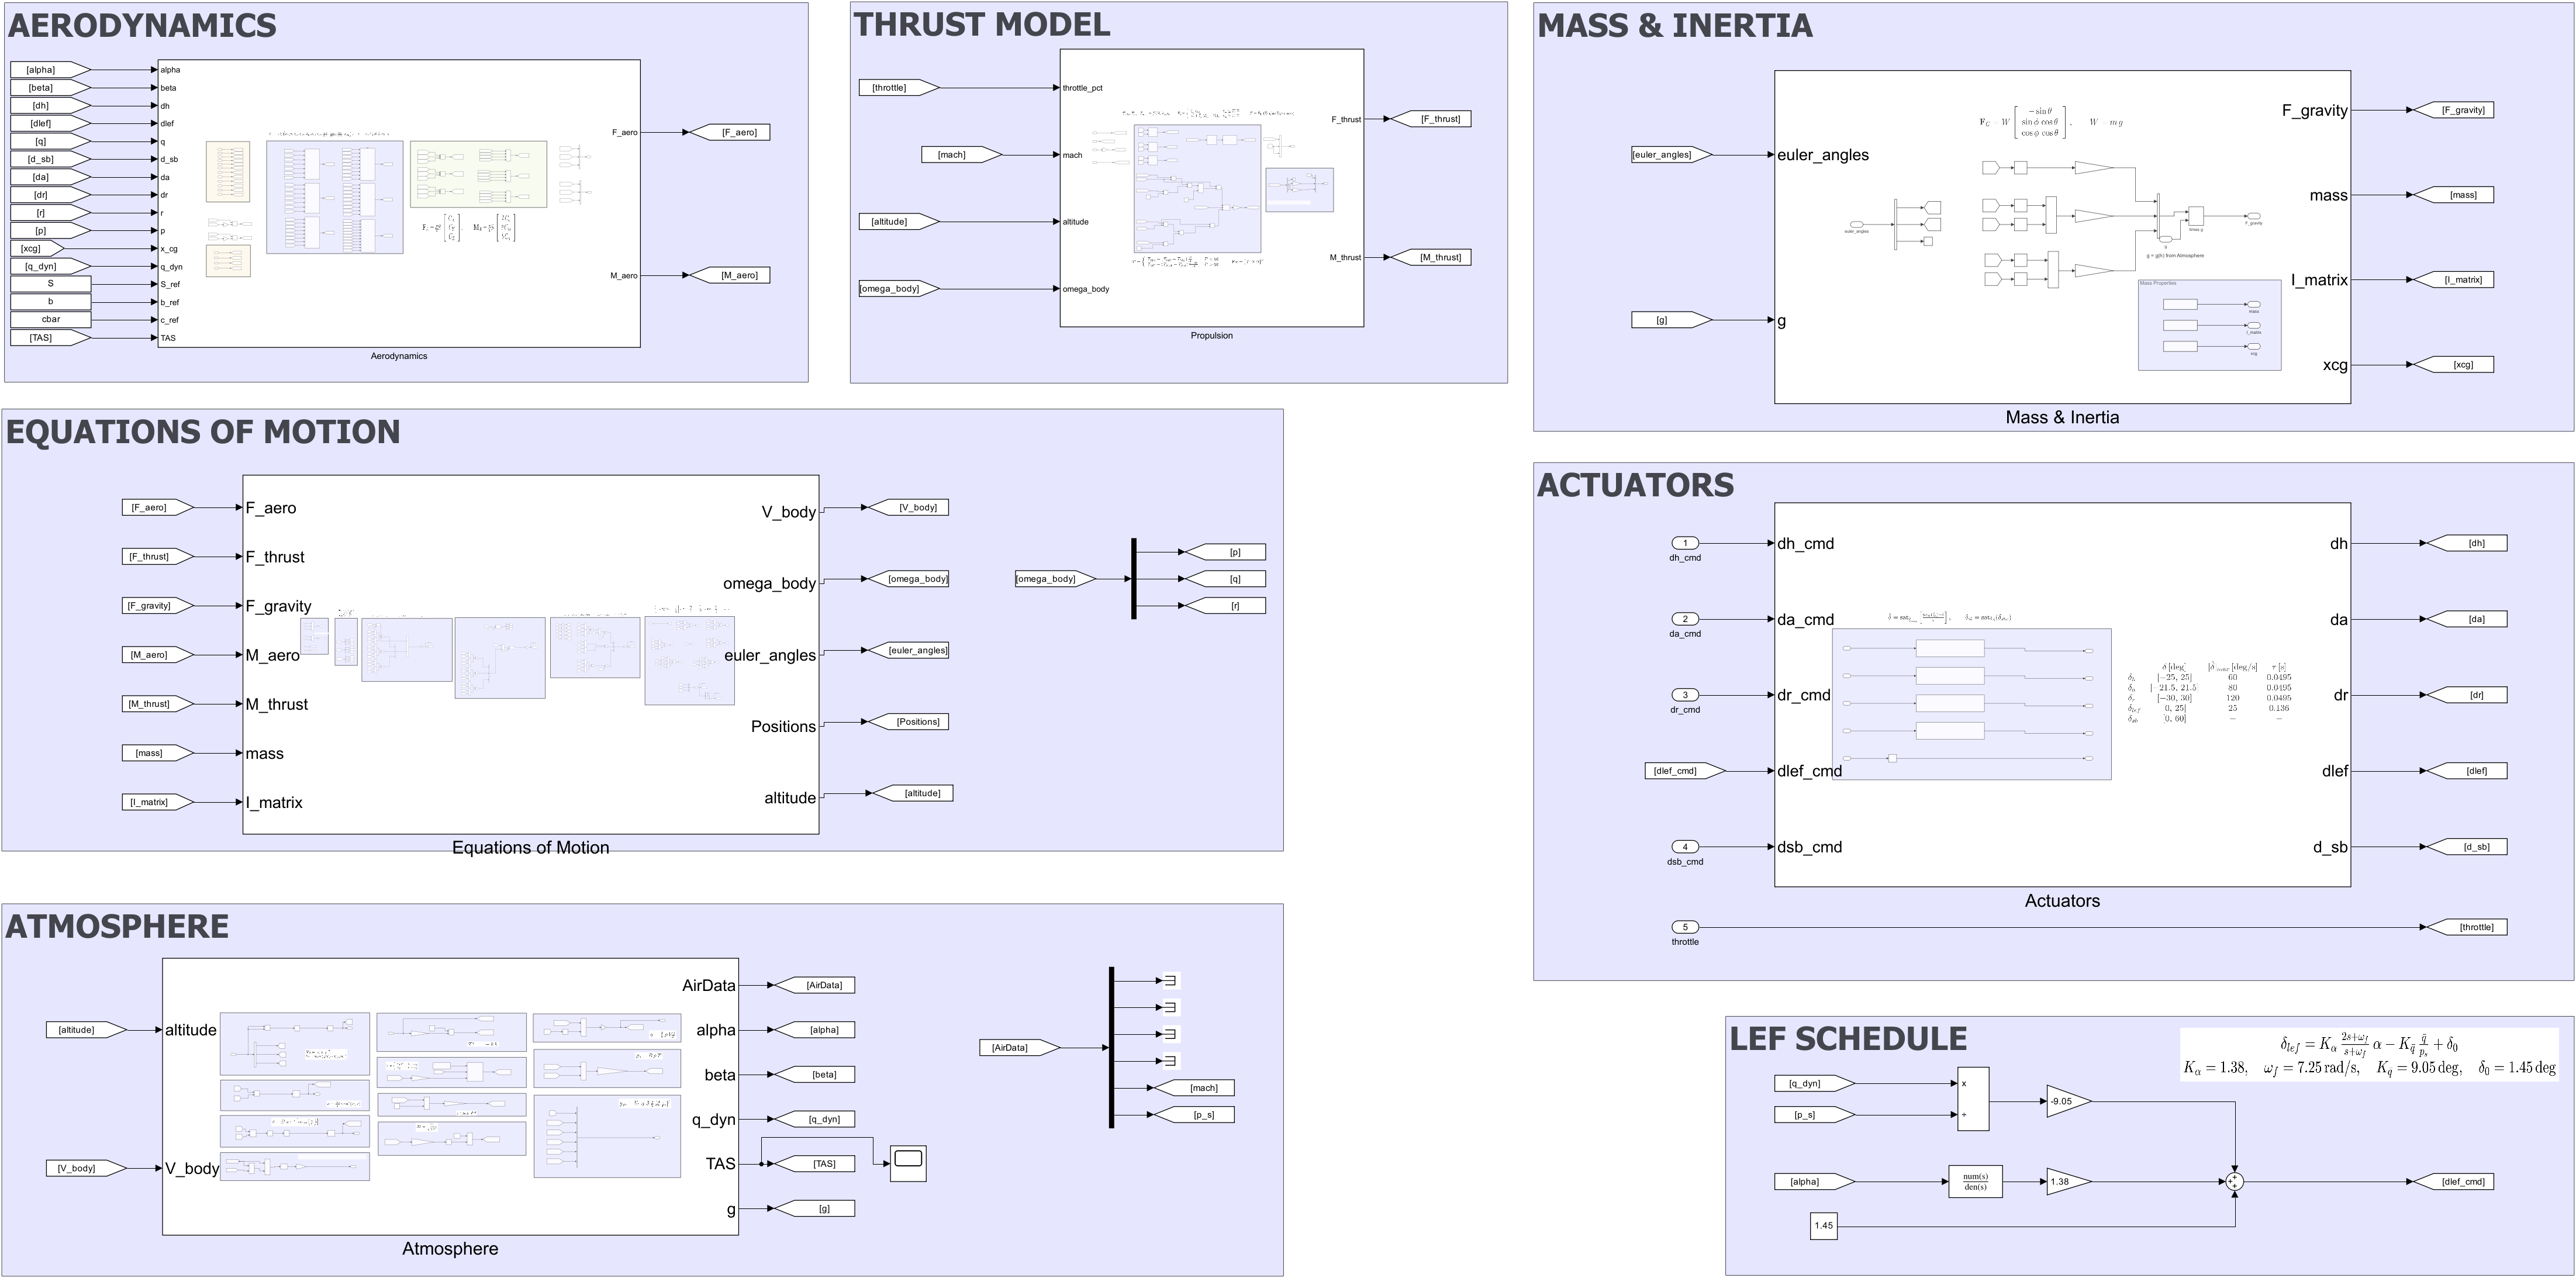
\includegraphics[width=\textwidth]{figures/MT_RootModel.png}
\caption{Bölüm~II.C'deki düzeltmelerden sonra F-16 Simulink modelinin kök seviyesi.}
\label{fig:model}
\end{figure}

\subsection{Alt sistemler}
\emph{Atmosfer.} Ref.~\cite{slj}, Ek A.6'daki standart atmosfer yoğunluğu, ses hızını, Mach sayısını, statik basıncı ve dinamik basıncı verir; $\alpha=\operatorname{atan2}(w,u)$ ve $\beta=\arcsin(v/V_T)$'dir. Alt sistem ayrıca yerçekimi ivmesini $g=g_0[R_e/(R_e+h)]^2$ olarak verir; $g_0=9,80665$~m/s$^2$, $R_e=6,371\times10^6$~m'dir.

\emph{Aerodinamik.} Gövde eksenindeki altı katsayı TP-1538'in yapısını izler~\cite{tp1538}: $\alpha$, $\beta$ ve $\delta_h$'ye bağlı temel tablolar, $(1-\delta_{lef}/25^\circ)$ ile ağırlıklandırılan LEF artımları, kumanda ve hava freni artımları ile $q\bar c/(2V_T)$, $pb/(2V_T)$ ve $rb/(2V_T)$'ye bağlı sönüm terimleri; toplam 68 arama tablosu. Veriler $0,35\bar c$'ye göre verilmiştir; momentler gerçek ağırlık merkezine $C_m \leftarrow C_m + C_Z(0,35-x_{cg})$ ve $C_n \leftarrow C_n - C_Y(0,35-x_{cg})\bar c/b$ ile taşınır~\cite{slj}.

\emph{İtki.} Gaz kolu dişlisi $\delta_T$'yi güç komutuna çevirir (\%77 askerî güce karşılık gelir); güce bağlı zaman sabitli birinci mertebe bir gecikme güç seviyesi $P_3$'ü verir ve itki, Mach sayısı ile irtifaya bağlı rölanti, askerî ve azami güç tabloları arasında aradeğerlenir~\cite{tp1538}. İtki $\mathbf F_T=[T\ 0\ 0]^T$, gövde $x$ ekseni boyunca ve ağırlık merkezinden etki eder. Alt sistem ayrıca motorun jiroskopik momentini verir: $\mathbf M_T=-\boldsymbol\omega\times\mathbf h_E=[0\ \ {-r}h_E\ \ qh_E]^T$, $\mathbf h_E=[h_E\ 0\ 0]^T$.

\emph{Kütle ve eylemsizlik.} Alt sistem, Atmosfer'den gelen $g$ ile yerçekimi kuvvetini $\mathbf F_G=mg[-\sin\theta\ \ \sin\phi\cos\theta\ \ \cos\phi\cos\theta]^T$ olarak hesaplar; ayrıca Aerodinamik alt sisteminin ve hareket denklemlerinin kullandığı kütleyi, eylemsizlik matrisini ve ağırlık merkezi konumunu verir.

\emph{Eyleyiciler.} Stabilatör, kanatçık, dümen ve LEF eyleyicilerinin her biri ayrı bir alt sistemdir; her biri konum ve hız sınırlı birinci mertebe bir gecikmedir (zaman sabitleri 0,0495~s, LEF için 0,136~s)~\cite{tp1538}.

\emph{Hareket denklemleri.} Düz ve dönmeyen bir Dünya üzerinde sabit kütleli rijit bir uçak için~\cite{slj}
\begin{equation}
m(\dot{\mathbf v}+\boldsymbol\omega\times\mathbf v)=\mathbf F_A+\mathbf F_T+\mathbf F_G, \qquad
\mathbf I\dot{\boldsymbol\omega}+\boldsymbol\omega\times\mathbf I\boldsymbol\omega=\mathbf M_A+\mathbf M_T
\label{eq:eom}
\end{equation}
yazılır; bunlara Euler açısı kinematiği ve kuzey--doğu--aşağı konum denklemleri eşlik eder. Kuvvet ve momentler bu alt sistemin içinde toplanır.

\emph{LEF tarifesi.} $\delta_{lef}=1,38\,\dfrac{2s+7,25}{s+7,25}\,\alpha-9,05\,\bar q/p_s+1,45$ (derece), $0$--$25^\circ$ aralığıyla sınırlıdır~\cite{slj}.

\subsection{Doğrulama ve düzeltmeler}
Aerodinamik ve İtki blokları test modellerinde ayrı ayrı çalıştırılmış; Ödev~1'deki on katsayı durumunun ve beş itki durumunun hepsinde bağımsız referans hesaplarıyla uyuşmuştur. Referans ağırlık merkezinde uçak küçük hücum açılarında yunuslamada statik olarak kararsızdır; statik marj yaklaşık $-\%4\,\bar c$'dir. Bu, TP-1538'de incelenen gevşetilmiş statik kararlılık konfigürasyonudur~\cite{tp1538}.

\emph{Düzeltmeler.} Ders verilerinde $C_{l_p}(\alpha=55^\circ)=-1200$ verilmiştir; veriler yüklenirken TP-1538'deki $-0,12$ değeriyle değiştirilir. Bu düzeltme Ödev~1'de yapılmıştır ve buradaki koşulları etkilemez ($\alpha<11^\circ$). Ödev~1 geri bildiriminden sonra model beş noktada düzeltilmiştir:
\begin{enumerate}
\item her eyleyici ayrı bir alt sistemdir (önceden tek blokta idiler);
\item yerçekimi ivmesi irtifaya bağlıdır ve Atmosfer alt sisteminin çıkışıdır (önceden sabit $g_0$ idi);
\item kütle, eylemsizlik matrisi ve ağırlık merkezi konumu Kütle ve Eylemsizlik alt sisteminin çıkışlarıdır (önceden hareket denklemlerinde ve kök seviyede doğrudan çalışma alanı sabitleri olarak kullanılıyordu);
\item motorun jiroskopik momenti İtki alt sisteminde hesaplanır (önceden hareket denklemlerindeydi);
\item kuvvet ve momentler Hareket Denklemleri alt sisteminde toplanır (önceden kök seviyede toplanıyordu).
\end{enumerate}
Geri bildirimin diğer maddeleri (LEF tarifesi ve eyleyicisi, yerçekimi kuvveti, motor dinamiği) modelde zaten vardı. $g$ sabit tutulduğunda düzeltilmiş model, keyfî durumlarda Ödev~1 modelinin durum türevlerini $6\times10^{-11}$ farkla verir; yani 1. ve 3--5. maddeler hiçbir sonucu değiştirmez. Tek fiziksel değişiklik $g(h)$'dir: 10\,000~ft'te $g$, $g_0$'dan \%0,1 küçüktür.

\section{Trim ve Doğrusallaştırma}

\subsection{Trim}
Trim problemi \texttt{fmincon} (SQP) ile çözülür. Bilinmeyenler $\alpha$, $\beta$, $\phi$, $\theta$, dönüş hızı $\dot\psi$ ve dört kumandadır; $V_T$ ve $h$ verilen Mach sayısı ile irtifadan hesaplanır. Kararlı dönüşte gövde hızları $p=-\dot\psi\sin\theta$, $q=\dot\psi\sin\phi\cos\theta$ ve $r=\dot\psi\cos\phi\cos\theta$ olup $\dot\phi=\dot\theta=0$ sağlanır. Maliyet fonksiyonu~\cite{slj}
\begin{equation}
J=\dot V_T^2+100(\dot\alpha^2+\dot\beta^2)+10(\dot p^2+\dot q^2+\dot r^2)
\end{equation}
uçuş yolu açısı kısıtı ve gerektiğinde yük faktörü kısıtı altında en küçüklenir. LEF her değerlendirmede kararlı hâl tarifesinden hesaplanır. Tablo~\ref{tab:trim} altı trim noktasını vermektedir. Bütün durumlarda $J<2\times10^{-11}$'dir ve modelin trimdeki türevleri (eyleyici, motor ve LEF filtresi durumları dahil) $10^{-4}$~m/s$^2$ ve $10^{-6}$~rad/s$^2$ düzeyinde sıfırdır. Bu raporun i, ii ve iii koşulları, sırasıyla Durum 1, 4 ve 6'dır.

\begin{table}[hbt!]
\caption{\label{tab:trim} Düzeltilmiş modelle yeniden hesaplanan Ödev~2 trim sonuçları (açılar derece, $\dot\psi$ rad/s)}
\centering
\small
\setlength\tabcolsep{3.5pt}
\begin{tabular}{clccccccccccc}
\toprule
Durum & $M$; $h$ [ft]; koşul & $x_{cg}$ & $V_T$ [m/s] & $\alpha$ & $\theta$ & $\phi$ & $\dot\psi$ & $\delta_T$ [\%] & $\delta_h$ & $\delta_a$ & $\delta_r$ & $\delta_{lef}$ \\
\midrule
\tabinput{tables/trim.tex}
\bottomrule
\end{tabular}
\end{table}

\subsection{Doğrusallaştırma}
Model her trim noktası etrafında merkezi farklarla, her seferinde bir durum veya giriş bozularak doğrusallaştırılır; türevler Simulink modelinden model API'si ile okunur. Bu raporda kullanılan rüzgâr ekseni modeli
\begin{equation}
\Delta\mathbf x=[\Delta V_T\ \Delta\alpha\ \Delta q\ \Delta\theta\ \Delta\beta\ \Delta p\ \Delta r\ \Delta\phi]^T,\qquad
\Delta\mathbf u=[\Delta\delta_T\ \Delta\delta_h\ \Delta\delta_a\ \Delta\delta_r]^T
\end{equation}
şeklindedir ve $A=\begin{bmatrix}A_{11}&A_{21}\\A_{12}&A_{22}\end{bmatrix}$; boyuna blok $A_{11}$, yanal-yönsel blok $A_{22}$ ve bağlaşım bloklarına ayrılır. Eyleyici ve motor durumları 8 durumlu modelde yer almaz; $\delta_{lef}$ trim değerinde sabit tutulur. Gövde ve rüzgâr ekseni modelleri, $T$ matrisi $[V_T,\alpha,\beta]$'nın $[u,v,w]$'ye göre Jacobian'ı olmak üzere, $A_W=TA_BT^{-1}$ bağıntısını $5\times10^{-6}$ bağıl farkla sağlar.

Şekil~\ref{fig:linnl}, iii koşulunda doğrusal ve doğrusal olmayan yanıtları karşılaştırır. Yanal kanallar örtüşür; boyuna kanalda ise doğrusal model ıraksarken doğrusal olmayan model ıraksamaz. Fark, doğrusal olmayan modelde $\alpha$'yı filtresi üzerinden geri besleyen LEF tarifesinden gelir. Eyleyici, motor ve LEF durumları dahil edildiğinde, iii trim noktasında tam doğrusal olmayan modelin özdeğerleri yalnızca $+0,044$~s$^{-1}$'lik yavaş bir kararsız kök içerir; LEF durumları dondurulduğunda 8 durumlu modelin $+0,788$~s$^{-1}$'lik kökü geri gelir.

\begin{figure}[hbt!]
\centering
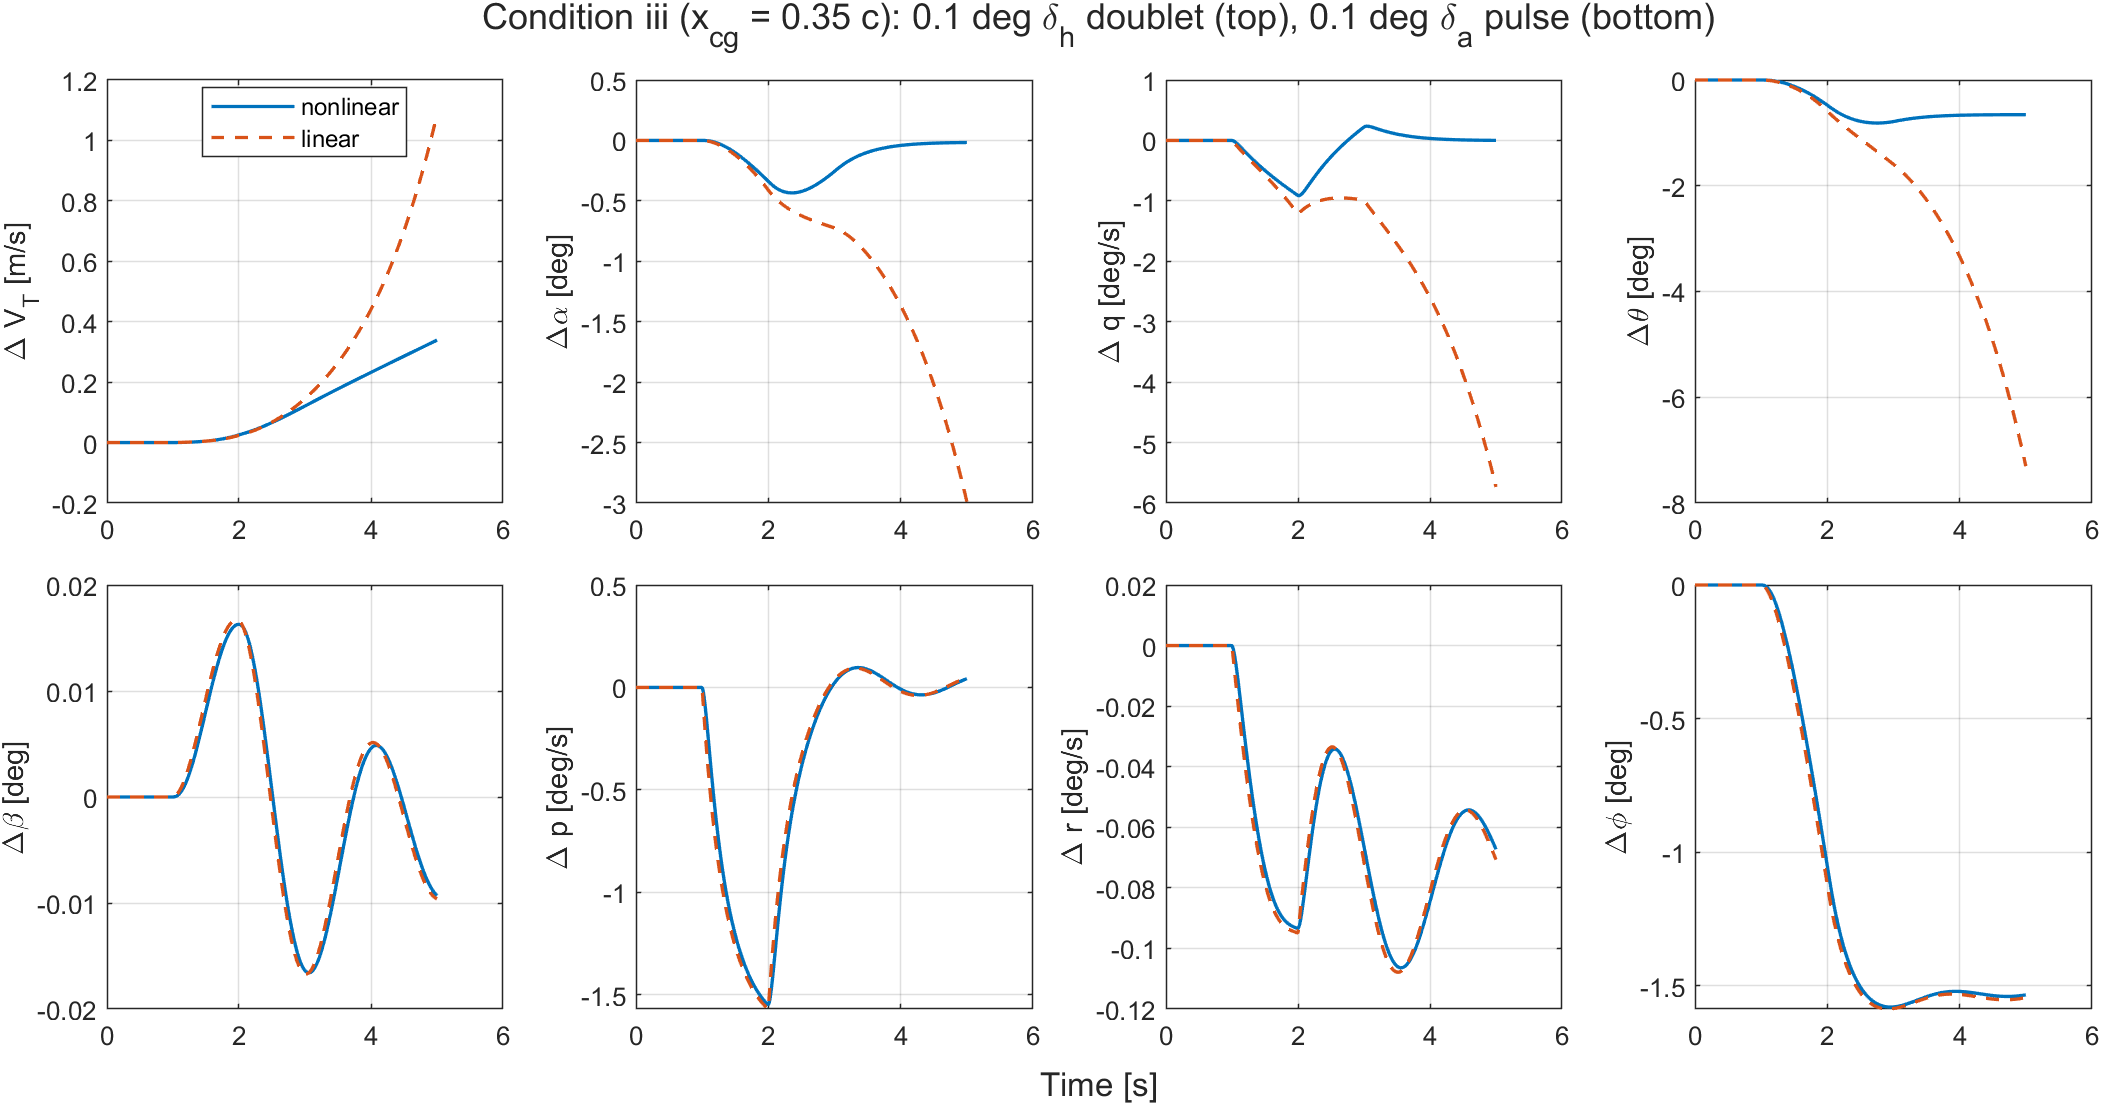
\includegraphics[width=0.95\textwidth]{figures/HW2_LinVsNonlin_iii.png}
\caption{iii koşulunda doğrusal (kesikli) ve doğrusal olmayan (sürekli) yanıtlar: $0,1^\circ$ stabilatör ikilisi (üst) ve $0,1^\circ$ kanatçık darbesi (alt).}
\label{fig:linnl}
\end{figure}

\emph{Düzeltmeler.} Trim ve doğrusallaştırma yöntemleri değişmemiştir; ancak Ödev~2'nin bütün sonuçları Bölüm~II.C'deki düzeltilmiş modelle yeniden hesaplanmıştır. Tablo~\ref{tab:trim} ve \texttt{HW2\_Group2.mat} yeni değerleri içerir. $g$ artık 10\,000~ft'te \%0,1 küçük olduğundan trim hücum açıları en fazla $0,01^\circ$, gaz kolu konumları en fazla \%0,04 azalır; $A_W$'nin elemanları en büyük elemanının en fazla $6\times10^{-4}$'ü kadar değişir. Durum 5'in yük faktörü yerel $g$ ile tanımlanmıştır. \texttt{run\_MT.m} i, ii ve iii koşullarında trimi ve doğrusallaştırmayı tekrarlar; elde edilen rüzgâr ekseni matrisleri yeniden hesaplanan \texttt{HW2\_Group2.mat}'takilerle aynıdır.

\section{Trim Uçuşu Benzetimi}

\subsection{Yöntem}
Doğrusal olmayan model her trim noktasından başlatılır: rijit cisim durumları trim çözümünden, eyleyici durumları trim açılarından, motor gücü trim gaz kolunun kararlı güç seviyesinden alınır ve LEF filtresi kararlı hâle yerleştirilir. Stabilatör, kanatçık, dümen ve gaz kolu komutları trim değerlerinde tutulur; $\delta_{lef}$ tarifeyi izler. Model değişken adımlı çözücüsüyle (en büyük adım 0,01~s) çözülür ve sonuçlar \texttt{Sim\_i}, \texttt{Sim\_ii} ve \texttt{Sim\_iii} için 0,01~s aralıklarla yeniden örneklenir. i ve iii koşulları 60~s, ii koşulu ise yön açısı $360^\circ$ değişene kadar koşturulur.

\subsection{Sonuçlar}
Şekil~\ref{fig:sim_i}--\ref{fig:sim_iii} zaman geçmişlerini, Tablo~\ref{tab:sim} ise trimden en büyük sapmaları göstermektedir. Kumanda girişleri benzetim boyunca trim değerlerinde kalır.

\begin{table}[hbt!]
\caption{\label{tab:sim} Benzetimler sırasında trimden en büyük sapmalar (açılar derece, hızlar derece/s)}
\centering
\begin{tabular}{ccccccccc}
\toprule
Koşul & Süre [s] & $|\Delta V_T|$ [m/s] & $|\Delta\alpha|$ & $|\Delta\beta|$ & $|\Delta\phi|$ & $|\Delta\theta|$ & $|\Delta q|$ & $|\Delta h|$ [m] \\
\midrule
\tabinput{tables/sim.tex}
\bottomrule
\end{tabular}
\end{table}

\emph{i koşulu.} Trim korunur: 60~s içinde hız $4\times10^{-4}$~m/s'den, duruş yaklaşık $10^{-4}$ dereceden, irtifa ise 1~cm'den az değişir. Kalan küçük hareket Bölüm~VI'daki modları gösterir. $V_T$, $\theta$ ve $h$ yaklaşık 45~s'lik yarım periyotla yavaşça salınır; bu, fugoid modudur (periyot 101~s). Yuvarlanma ve sapma hızlarında ilk 10~s içinde yaklaşık 1,8~s periyotlu sönümlü bir salınım görülür; bu, Hollanda yuvarlanmasıdır (1,84~s). Yatış açısı kararlı spiral modun zaman ölçeğinde ($\tau=89$~s) tek yönlü kayar. Hareketi trim artıkları ve çözücünün başlangıcı uyarır; bütün modlar kararlı olduğundan hareket sınırlı kalır.

\emph{ii koşulu.} Bir tam dönüş 73,05~s sürer; trim çözümünden bulunan değer $2\pi/\dot\psi_1=73,04$~s'dir. Yer izi (Şekil~\ref{fig:track}) 2289~m yarıçaplı kapalı bir çemberdir; $V_T^2/(g\tan\phi)$ bağıntısı 2285~m verir. İrtifa 9~cm değişir. Yunuslama açısı ve sapma hızı yaklaşık 50~s periyotla salınır; bu değer tam modelin bağlaşık fugoid--spiral modunun 57~s'lik periyoduna yakındır (Bölüm~VI). Hollanda yuvarlanması geçici yanıtı yine 10~s içinde söner.

\emph{iii koşulu.} Sapmalar salınım yapmadan tek yönlü büyür: yunuslama açısı 20, 40 ve 60~s'de sırasıyla $5,1\times10^{-4}$, $1,7\times10^{-3}$ ve $3,9\times10^{-3}$ derece değişir; uçak yavaşça burun aşağı döner, hızlanır ve alçalır. 40 ile 60~s arasındaki büyüme hızı yaklaşık 0,04~s$^{-1}$'dir. Bu değer, LEF tarifesi etkin tam modelin $+0,044$~s$^{-1}$'lik yavaş kararsız köküyle (iki katına çıkma süresi yaklaşık 16~s) uyumludur (Bölüm~III). LEF sabit 8 durumlu modelin $+0,787$~s$^{-1}$'lik köküyle (Bölüm~VI) ise uyumlu değildir; o kök bir bozuntuyu 60~s'de $e^{47}$ katına çıkarırdı. Dolayısıyla iii koşulunun trimi kararsız bir denge noktasıdır; sapmaların küçük kalmasının tek nedeni, başlangıç bozuntusunun trim artıkları mertebesinde olmasıdır.

\begin{figure}[hbt!]
\centering
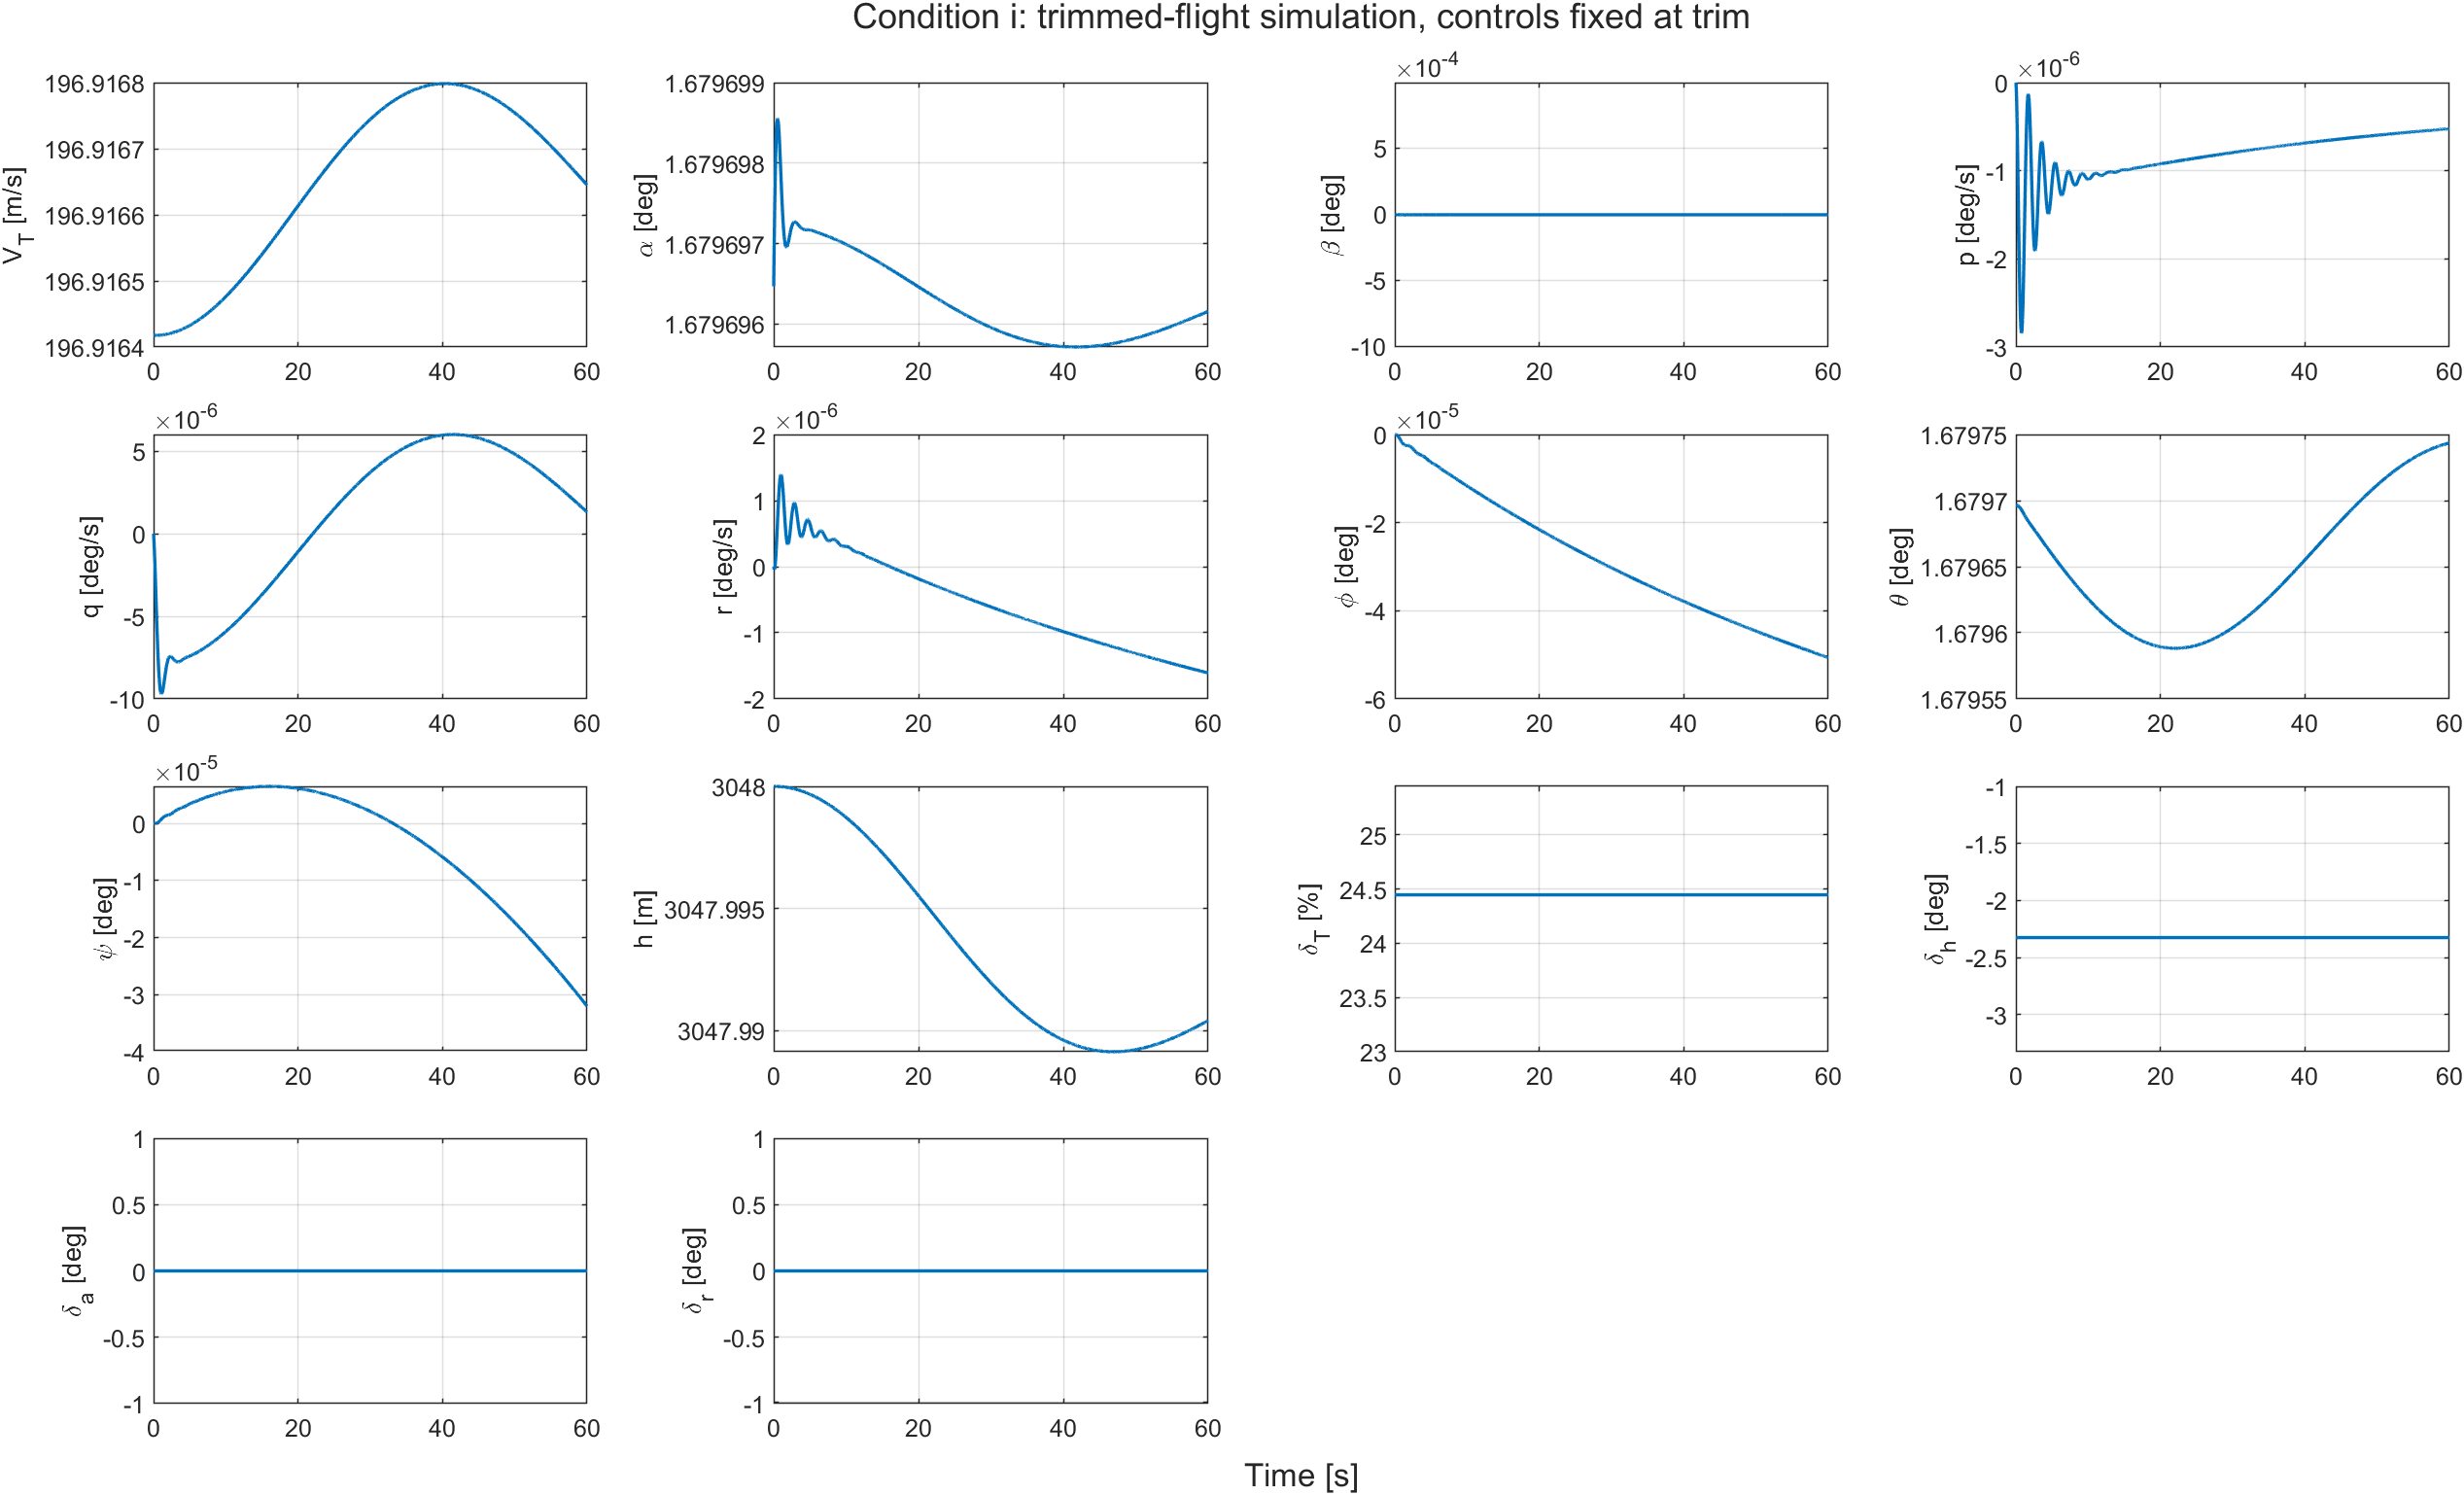
\includegraphics[width=\textwidth]{figures/MT_Sim_i.png}
\caption{Trim uçuşu benzetimi, i koşulu (kumandalar trimde sabit).}
\label{fig:sim_i}
\end{figure}

\begin{figure}[hbt!]
\centering
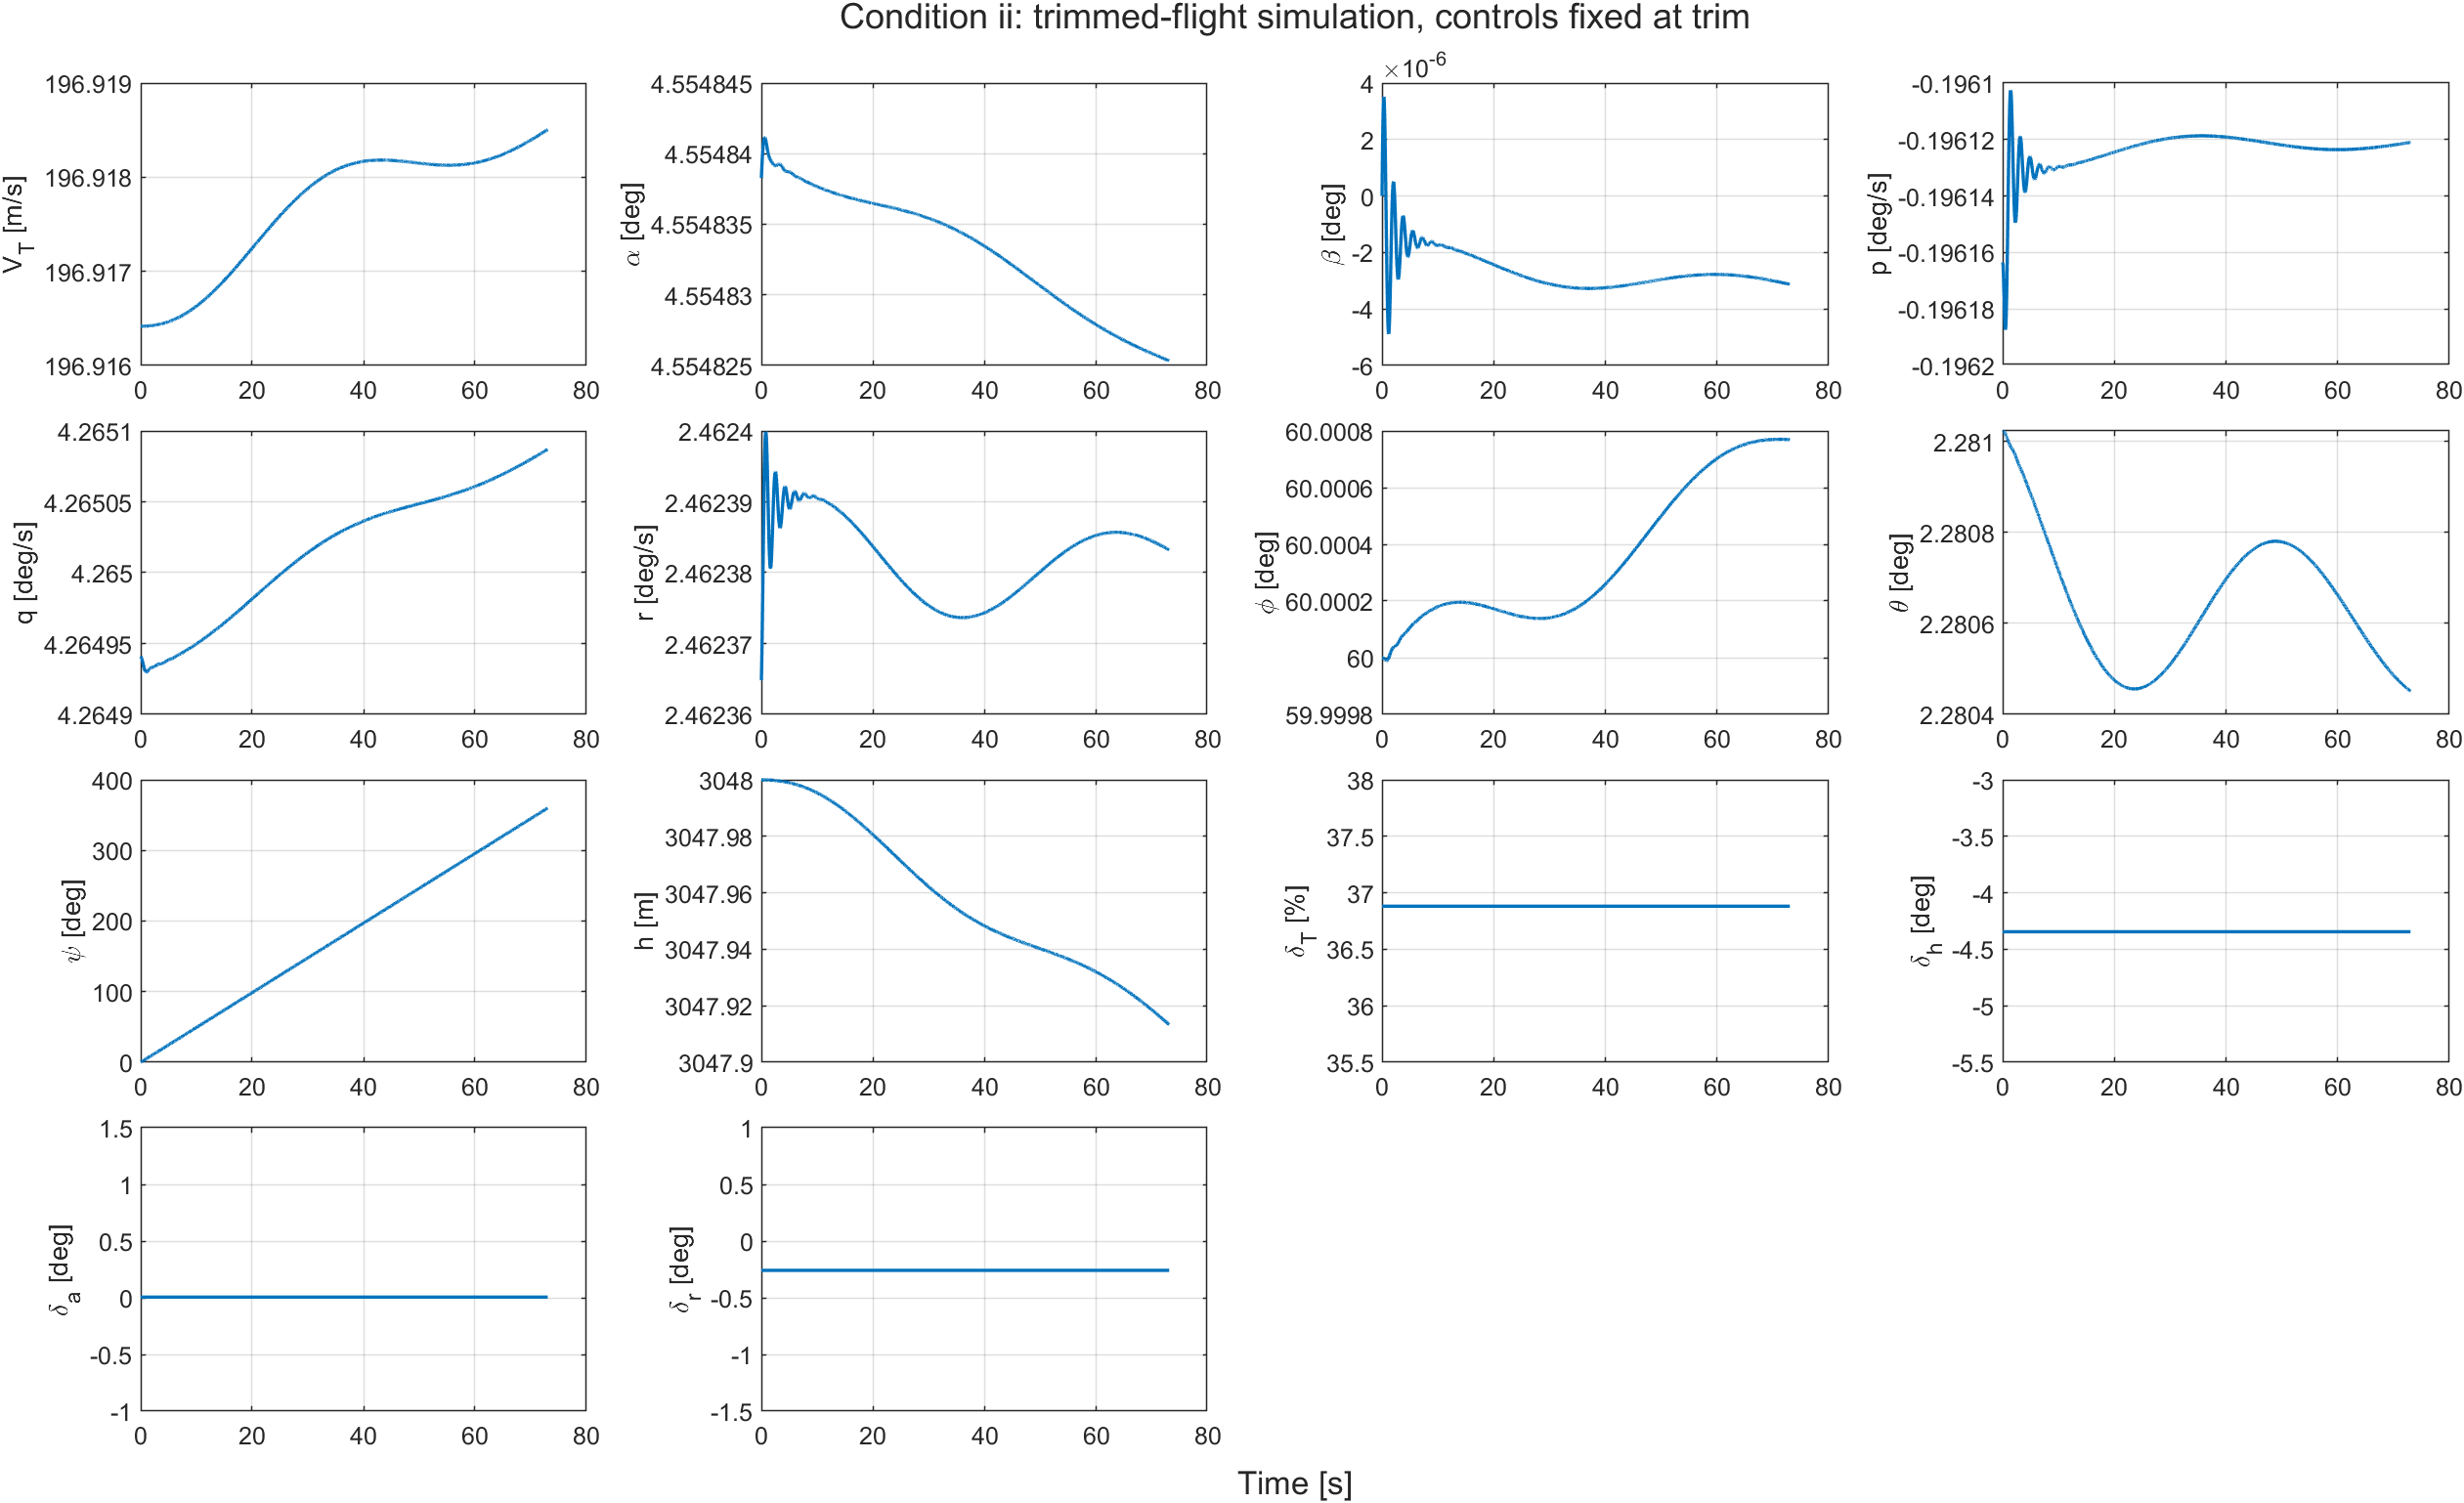
\includegraphics[width=\textwidth]{figures/MT_Sim_ii.png}
\caption{Trim uçuşu benzetimi, ii koşulu (bir tam dönüş).}
\label{fig:sim_ii}
\end{figure}

\begin{figure}[hbt!]
\centering
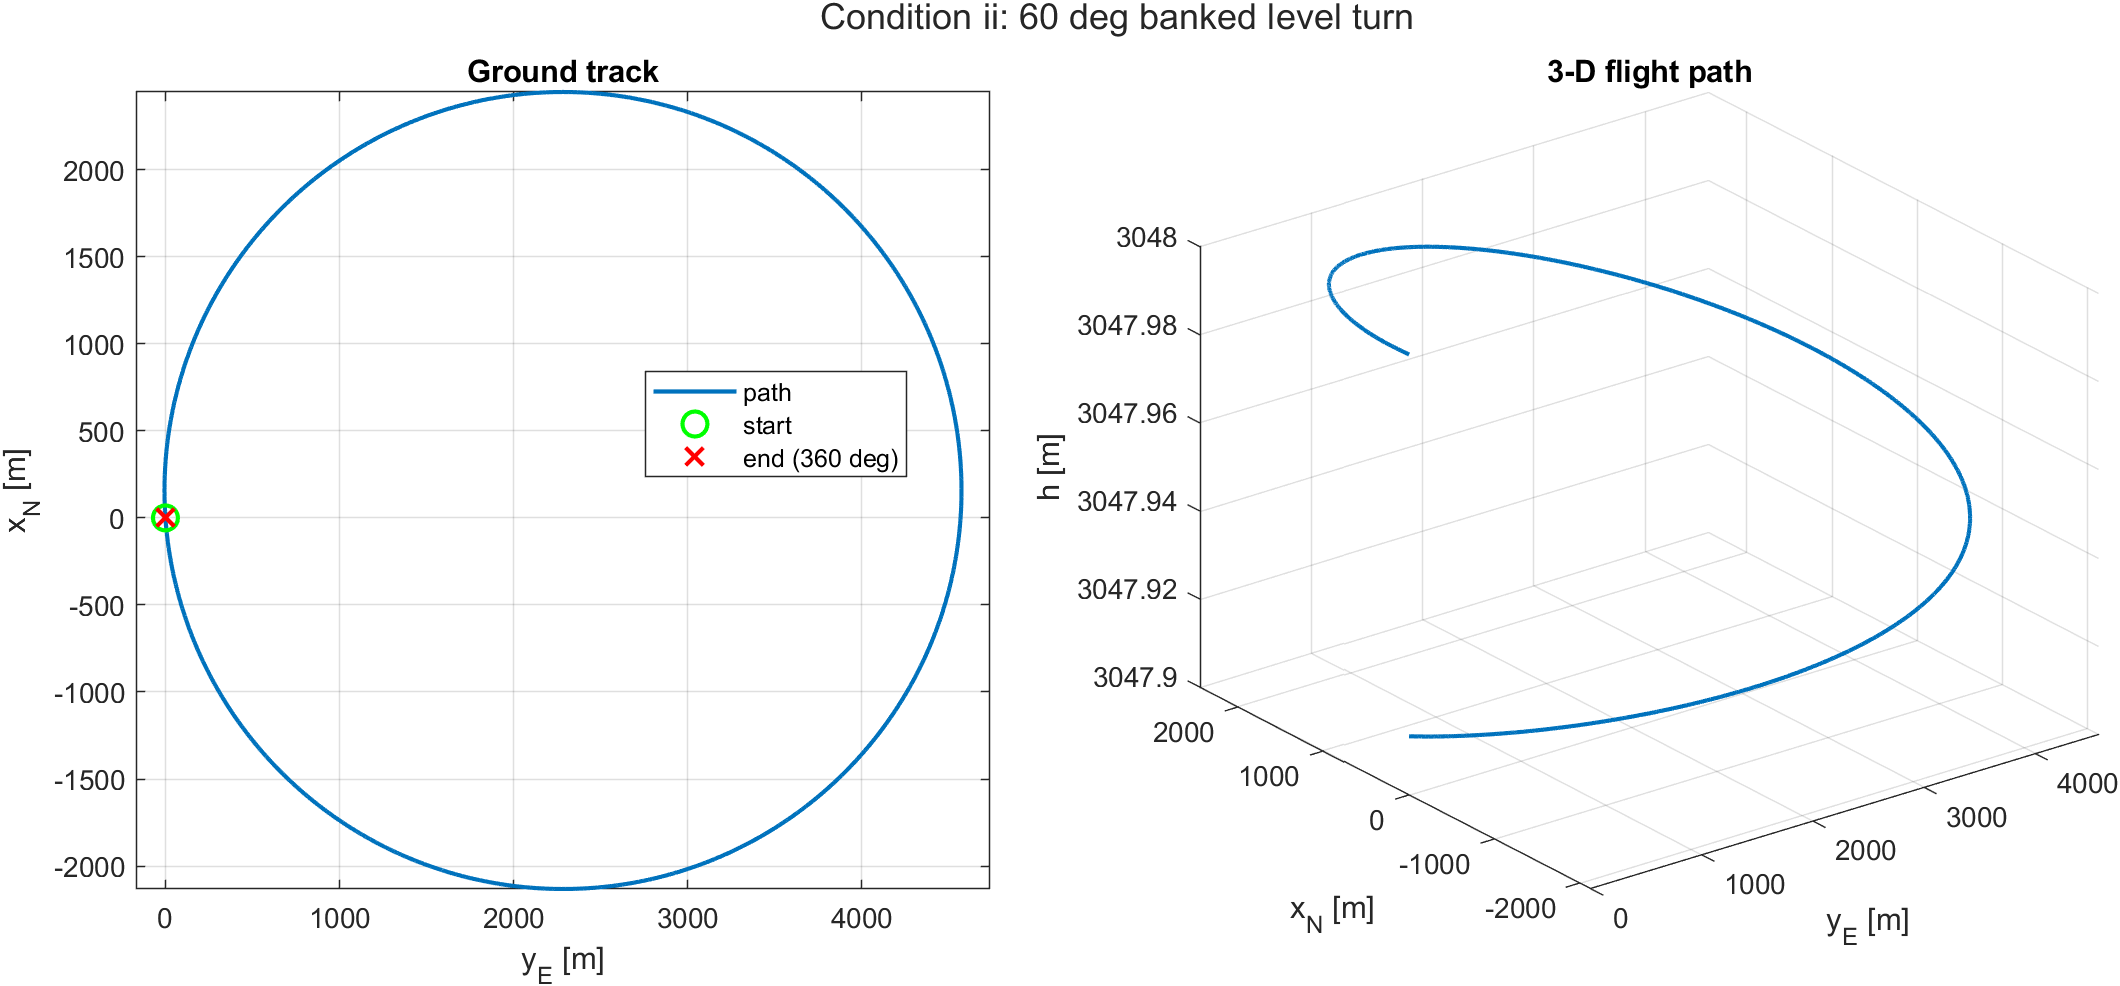
\includegraphics[width=0.85\textwidth]{figures/MT_Track_ii.png}
\caption{ii koşulunda yer izi ve üç boyutlu uçuş yolu (irtifa ekseni büyütülmüştür).}
\label{fig:track}
\end{figure}

\begin{figure}[hbt!]
\centering
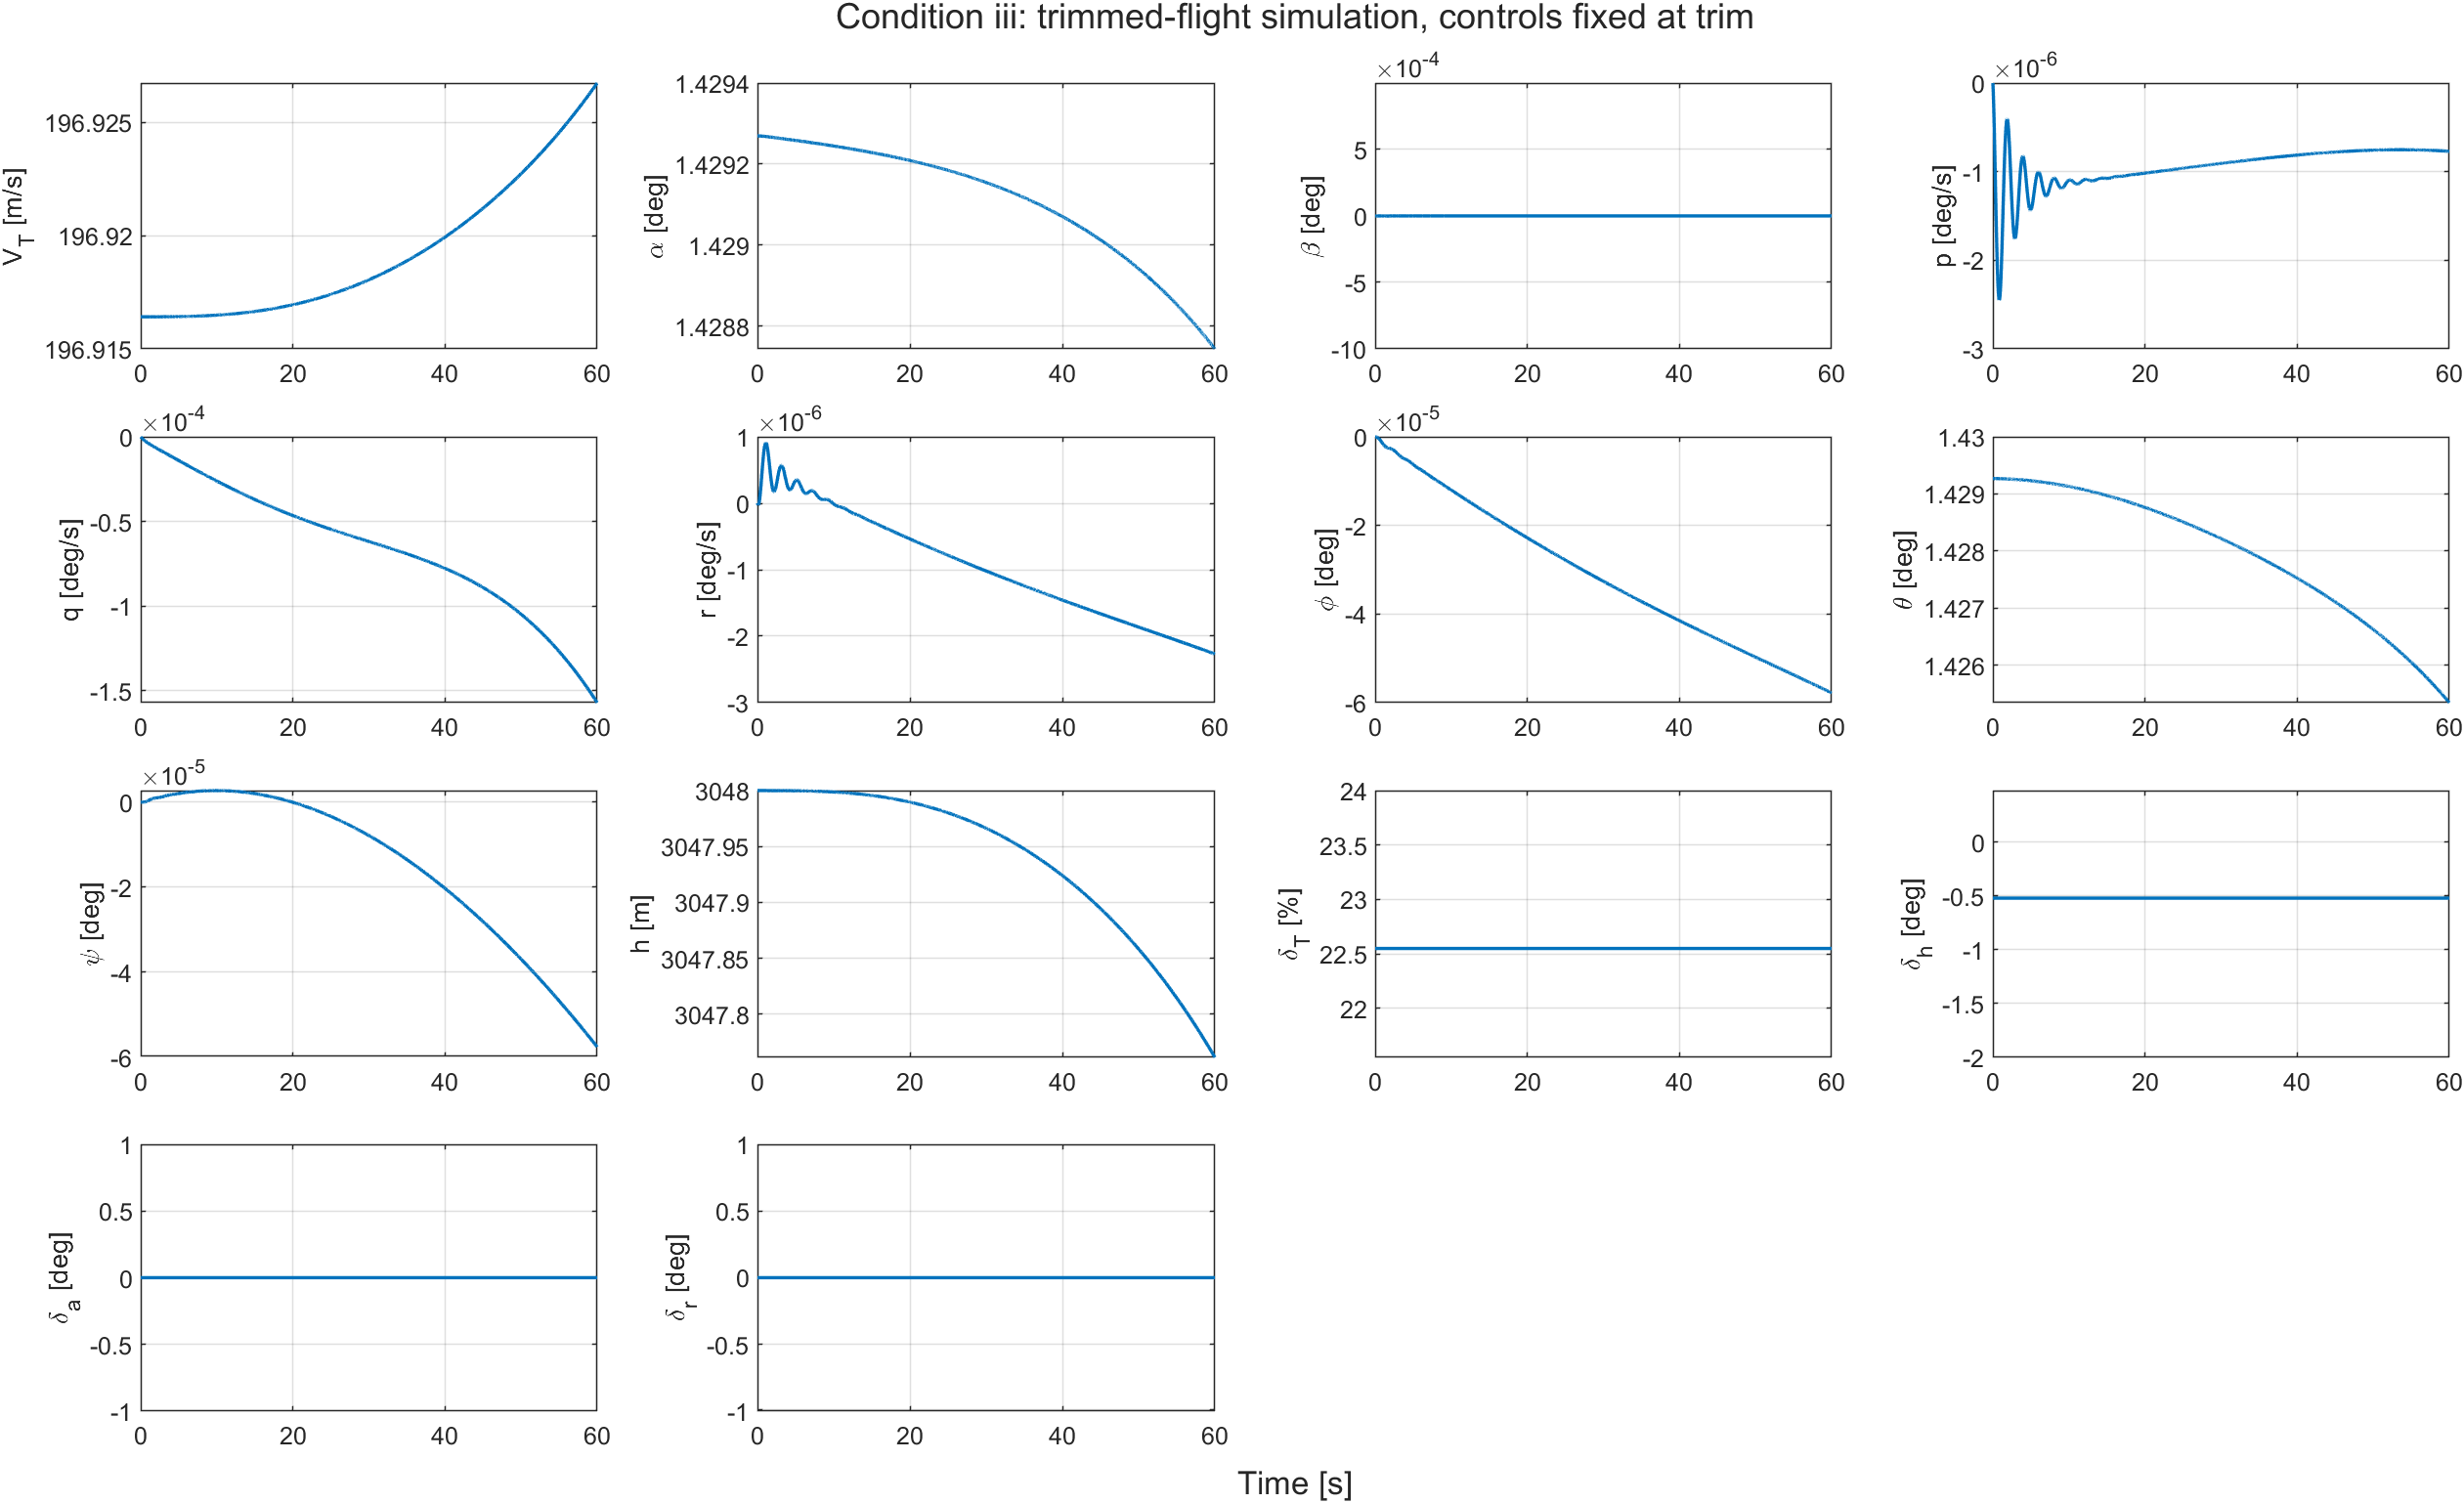
\includegraphics[width=\textwidth]{figures/MT_Sim_iii.png}
\caption{Trim uçuşu benzetimi, iii koşulu (kumandalar trimde sabit).}
\label{fig:sim_iii}
\end{figure}

\section{Kararlılık Parametreleri}

\subsection{Bağıntılar}
Ders~6'nın~\cite{lec6} boyuna durum değişkeni modeli (s.~24--25), $\Delta u$ yerine $\Delta V_T$ ve trimde $U_1=V_T$ alınarak
\begin{equation}
a_{11}=X_u+X_{T_u},\quad
a_{31}=(M_u+M_{T_u})-\frac{M_{\dot\alpha}Z_u}{Z_{\dot\alpha}-U_1},\quad
a_{32}=(M_\alpha+M_{T_\alpha})-\frac{M_{\dot\alpha}Z_\alpha}{Z_{\dot\alpha}-U_1},\quad
a_{33}=M_q-\frac{M_{\dot\alpha}(Z_q+U_1)}{Z_{\dot\alpha}-U_1}
\end{equation}
verir. Yanal-yönsel modelde (s.~100--101) yuvarlanma ve sapma satırları eylemsizlik bağlaşımını içerir:
\begin{equation}
a_{6k}=\frac{L_k+(I_{xz}/I_{xx})N_k}{1-I_{xz}^2/(I_{xx}I_{zz})},\qquad
a_{7k}=\frac{N_k+(I_{xz}/I_{zz})L_k}{1-I_{xz}^2/(I_{xx}I_{zz})},\qquad k=\beta,p,r.
\end{equation}
Bu bağıntı
\begin{equation}
L_k=a_{6k}-\frac{I_{xz}}{I_{xx}}\,a_{7k},\qquad N_k=a_{7k}-\frac{I_{xz}}{I_{zz}}\,a_{6k}
\label{eq:invert}
\end{equation}
şeklinde ters çevrilir. $p$ ve $r$ gövde ekseni hızları olduğundan Bölüm~II'deki gövde ekseni eylemsizlikleri kullanılır ve elde edilen türevler gövde ekseni türevleridir. Boyutsuz türevler Ders~5'teki~\cite{lec5} tanımlardan (s.~116 ve 123) bulunur:
\begin{gather}
X_u=-\frac{\bar q_1S}{mU_1}(C_{D_u}+2C_{D_1}),\quad
M_u=\frac{\bar q_1S\bar c}{I_{yy}U_1}(C_{m_u}+2C_{m_1}),\quad
M_\alpha=\frac{\bar q_1S\bar c}{I_{yy}}C_{m_\alpha},\quad
M_q=\frac{\bar q_1S\bar c^2}{2I_{yy}U_1}C_{m_q},\\
L_\beta=\frac{\bar q_1Sb}{I_{xx}}C_{l_\beta},\quad
N_\beta=\frac{\bar q_1Sb}{I_{zz}}C_{n_\beta},\quad
L_{p,r}=\frac{\bar q_1Sb^2}{2I_{xx}U_1}C_{l_{p,r}},\quad
N_{p,r}=\frac{\bar q_1Sb^2}{2I_{zz}U_1}C_{n_{p,r}}.
\end{gather}
Üç koşulda da $U_1=196,92$~m/s ve $\bar q_1=17\,564$~Pa'dır.

\emph{İtki.} İtki gövde $x$ ekseni boyunca etki ettiğinden $\dot V_T$'ye katkısı $T\cos\alpha\cos\beta/m$'dir ve
\begin{equation}
X_{T_u}=\frac{\cos\alpha_1\cos\beta_1}{m}\frac{\partial T}{\partial V_T}\bigg|_{\delta_T,h}
\end{equation}
olur. Türev, uçak modelinin İtki bloğu tek başına, trim gaz kolu ve irtifasında, motor kararlı hâldeyken $M=0,6\pm0,001$'de çalıştırılarak hesaplanır. Böylece $X_u=a_{11}-X_{T_u}$ bulunur.

\emph{Trim katsayıları.} Trimdeki $\dot V_T$ denkleminden $C_{D_1}=(T_1\cos\alpha_1\cos\beta_1-mg\sin\gamma_1)/(\bar q_1S)$ elde edilir. Denk.~(\ref{eq:eom}) $\dot{\boldsymbol\omega}=0$ ve $\mathbf M_T=-\boldsymbol\omega\times\mathbf h_E$ ile yazıldığında trimdeki aerodinamik yunuslama momenti eylemsizlik ve jiroskopik momentleri dengeler: $C_{m_1}=[\boldsymbol\omega_1\times(\mathbf I\boldsymbol\omega_1+\mathbf h_E)]_y/(\bar q_1S\bar c)$. Tablo~\ref{tab:p2trim} bu büyüklükleri, Tablo~\ref{tab:aelem} kullanılan $A$ elemanlarını, Tablo~\ref{tab:params} ve \ref{tab:derivs} ise sonuçları vermektedir.

\begin{table}[hbt!]
\caption{\label{tab:p2trim} Türevler için kullanılan trim büyüklükleri}
\centering
\begin{tabular}{ccccc}
\toprule
Koşul & $T_1$ [N] & $\partial T/\partial V_T$ [N\,s/m] & $C_{D_1}$ & $C_{m_1}$ \\
\midrule
\tabinput{tables/p2trim.tex}
\bottomrule
\end{tabular}
\end{table}

\begin{table}[hbt!]
\caption{\label{tab:aelem} Problem 2'de kullanılan rüzgâr ekseni $A$ matrisi elemanları}
\centering
\begin{tabular}{llccc}
\toprule
Eleman & Birim & i & ii & iii \\
\midrule
\tabinput{tables/aelem.tex}
\bottomrule
\end{tabular}
\end{table}

\begin{table}[hbt!]
\caption{\label{tab:params} Kararlılık parametreleri (\texttt{StabParams})}
\centering
\begin{tabular}{llccc}
\toprule
Parametre & Birim & i & ii & iii \\
\midrule
\tabinput{tables/params.tex}
\bottomrule
\end{tabular}
\end{table}

\begin{table}[hbt!]
\caption{\label{tab:derivs} Boyutsuz kararlılık türevleri (\texttt{StabDerivs}, rad$^{-1}$) ve olağan işaretleri~\cite{lec5}}
\centering
\begin{tabular}{lcccc}
\toprule
Türev & i & ii & iii & Olağan işaret \\
\midrule
\tabinput{tables/derivs.tex}
\bottomrule
\end{tabular}
\end{table}

\subsection{Modelde sıfır olan terimler}
\begin{itemize}
\item $Z_{\dot\alpha}=M_{\dot\alpha}=0$: TP-1538 verilerinde $\dot\alpha$ türevleri yoktur; bu nedenle $a_{31}$, $a_{32}$ ve $a_{33}$'teki düzeltme terimleri sıfırdır ve $a_{32}=M_\alpha+M_{T_\alpha}$, $a_{33}=M_q$ olur.
\item $M_{T_u}=M_{T_\alpha}=0$ ve $N_{T_\beta}=0$: itki gövde $x$ ekseni boyunca ve ağırlık merkezinden etki eder, $\alpha$ veya $\beta$'ya bağlı değildir; motor modelinde hava alığı momentum terimleri yoktur.
\item $C_{D_u}$ ve $C_{m_u}$ düz uçuşta (i ve iii) sıfırdır ($10^{-9}$ mertebesinde, yani sayısal sıfır): aerodinamik tablolar Mach sayısına bağlı olmadığından sabit $\alpha$'da hız değişimi kuvvet ve momentleri yalnızca $\bar q$ ile ölçekler; bu etki $2C_{D_1}$ ve $2C_{m_1}$ terimlerinde zaten vardır. Aynı nedenle düz uçuşta $C_{m_1}=0$'dır; orada yalnızca aerodinamik moment dengelenir.
\item $X_{T_u}$ sıfır değildir: bu koşulda itki Mach sayısıyla hafifçe azalır ($\partial T/\partial V_T\approx-35$~N\,s/m); böylece i koşulunda motor hız sönümüne yaklaşık \%23 katkı yapar.
\end{itemize}
Buna karşılık ders modeli $C_{D_q}\approx0$ (yani $X_q=0$) kabul eder; F-16 verilerinde eksenel kuvvette sönüm terimleri bulunduğundan $a_{13}=\partial\dot V_T/\partial q=-0,138$~(m/s)/(rad/s) elemanı sıfır değildir.

\subsection{İşaretler ve statik kararlılık}
i ve ii koşullarında bütün türevler olağan işaretlerine sahiptir; olağan işareti tanımlı olmayan türevler ($C_{D_u}$, $C_{m_u}$, $C_{n_p}$) küçüktür. iii koşulunda $C_{m_\alpha}=+0,156$~rad$^{-1}$'in işareti terstir. Dolayısıyla uçak
\begin{itemize}
\item i ve ii koşullarında yunuslama, yuvarlanma ve sapmada statik olarak kararlıdır ($C_{m_\alpha}<0$, $C_{l_\beta}<0$, $C_{n_\beta}>0$);
\item iii koşulunda yunuslamada statik olarak kararsız, yuvarlanma ve sapmada ise kararlıdır.
\end{itemize}
i ile iii arasındaki fark, Bölüm~II'deki $C_m\leftarrow C_m+C_Z(0,35-x_{cg})$ moment taşımasıdır; bu terim $x_{cg}=0,35$'te sıfırlanır. Terim $C_{m_\alpha}$'yı $0,10\,C_{Z_\alpha}=-0,386$~rad$^{-1}$ kadar kaydırır; buradan $C_{Z_\alpha}\approx-3,86$~rad$^{-1}$ ve nötr nokta yaklaşık $0,35-0,156/3,86\approx0,31\bar c$ bulunur. Bu, Ödev~1'de bulunan $-\%4\,\bar c$'lik statik marjla uyumludur. Aynı terim $C_{m_q}$'ya $0,10\,C_{Z_q}$ ekler; öndeki ağırlık merkezinde yunuslama sönümünün daha büyük olmasının ($-8,22$'ye karşı $-5,23$) nedeni budur. $0,35\bar c$'de dikey kuyruğun moment kolunun kısalması da $C_{n_\beta}$'yı 0,219'dan 0,181'e düşürür.

\subsection{ii koşulu}
Ders~5'teki bağıntılar $p_1=q_1=r_1=\phi_1=0$ olan kararlı düz uçuş için türetilmiştir (s.~13 ve 16). Dönüşte değerler üç nedenle farklıdır.

\emph{Aerodinamik durum.} Trim hücum açısı $1,68^\circ$ yerine $4,55^\circ$, $\delta_{lef}$ ise $1,49^\circ$ yerine $5,45^\circ$'tir; dolayısıyla tablolar farklı bir noktada okunur. Dihedral etkisi $\alpha$ ile büyür ($C_{l_\beta}$: $-0,102$'den $-0,134$'e); kaldırma ile ölçeklenen $C_{l_r}$ de büyür.

\emph{Eylemsizlik terimleri.} $\boldsymbol\omega_1\neq0$ olduğunda hareket denklemlerindeki (Denk.~\ref{eq:eom}) $\boldsymbol\omega\times\mathbf I\boldsymbol\omega$ eylemsizlik teriminin ve motor momenti $\mathbf M_T$'nin, yani birlikte $\boldsymbol\omega\times(\mathbf I\boldsymbol\omega+\mathbf h_E)$ teriminin, $p$, $q$ ve $r$'ye göre Jacobian'ı sıfır değildir ve $A$'nın hız sütunlarında aerodinamik sönümle birlikte görünür. Denk.~(\ref{eq:invert}) $I_{xz}$ bağlaşımını ayırır, ancak bu terimleri ayırmaz. En büyüğü $\partial[\boldsymbol\omega\times\mathbf I\boldsymbol\omega]_z/\partial p=(I_{yy}-I_{xx})q_1=4,67\times10^{3}$~N\,m\,s'dir ve $C_{n_p}$'nin işaretini değiştirir. Jacobian $\mathbf I A$'ya geri eklendiğinde yalnızca aerodinamik kısım elde edilir (Tablo~\ref{tab:turnaero}); \texttt{StabDerivs} ise istendiği gibi doğrudan $A$'dan bulunan değerleri içerir.

\emph{Trimdeki açısal hız terimleri.} $q_1$ sabitken hız değiştiğinde $\hat q_1=q_1\bar c/(2U_1)$ değişir; bu yüzden sönüm terimleri $C_{m_u}$ ve $C_{D_u}$'yu sıfırdan farklı yapar: $C_{m_u}=-C_{m_q}\hat q_1=8,37\times6,52\times10^{-4}=0,0055$ (Tablo~\ref{tab:derivs}). Trimdeki eylemsizlik kaynaklı yunuslama momenti küçüktür: $C_{m_1}=1,0\times10^{-5}$.

\begin{table}[hbt!]
\caption{\label{tab:turnaero} ii koşulunda sönüm türevleri: $A$'dan ve yalnızca aerodinamik kısım (rad$^{-1}$)}
\centering
\begin{tabular}{lcccc}
\toprule
 & $C_{l_p}$ & $C_{n_p}$ & $C_{l_r}$ & $C_{n_r}$ \\
\midrule
\tabinput{tables/turnaero.tex}
\bottomrule
\end{tabular}
\end{table}

\section{Dinamik Modlar}

\subsection{Yöntem}
Her koşulda tam $A$ matrisinin ve $A_{11}$ ile $A_{22}$ bloklarının özdeğerleri hesaplanır. $\lambda=-\zeta\omega_n\pm j\omega_n\sqrt{1-\zeta^2}$ karmaşık eşleniği için $\omega_n=|\lambda|$, $\zeta=-\operatorname{Re}\lambda/|\lambda|$, periyot $2\pi/|\operatorname{Im}\lambda|$ ve $\tau=-1/\operatorname{Re}\lambda$'dır; gerçel bir kök için $\tau=-1/\lambda$'dır. Genliğin yarıya inme ve iki katına çıkma süreleri $t_{1/2}=\tau\ln2$ ($\tau>0$) ve $t_2=-\tau\ln2$ ($\tau<0$) ile bulunur~\cite{lec6}. Tam modelde modlar özvektörlerden belirlenir: $\Delta V_T$, $1/U_1$ ile ölçeklendikten sonra bir özvektörün boyuna payı, kare normunun ilk dört durumdaki kesridir. Hollanda yuvarlanması, boyuna payı en küçük karmaşık eşleniktir; diğer eşleniklerden hızlı olanı kısa periyot, yavaş olanı fugoiddir; kalan iki gerçel kökten hızlı olanı yuvarlanma, yavaş olanı spiral moddur. Kısa periyodun iki gerçel köke ayrıldığı iii koşulunda bu kökler, boyuna payı en büyük iki gerçel köktür; \texttt{Modes\_Full} ve \texttt{Modes\_Dec}'e kararsız kök yazılmıştır.

\begin{table}[hbt!]
\caption{\label{tab:modes} Tam $8\times8$ modelin modları (\texttt{Modes\_Full}); süreler s, $\omega_n$ rad/s}
\centering
\small
\begin{tabular}{cllcccccc}
\toprule
Koşul & Mod & $\lambda$ [s$^{-1}$] & $\omega_n$ & $\zeta$ & Periyot & $\tau$ & $t_{1/2}$ & $t_2$ \\
\midrule
\tabinput{tables/modes.tex}
\bottomrule
\end{tabular}
\end{table}

\begin{table}[hbt!]
\caption{\label{tab:modesdec} ii koşulunda ayrık $A_{11}$ ve $A_{22}$ bloklarının modları (\texttt{Modes\_Dec})}
\centering
\small
\begin{tabular}{llcccccc}
\toprule
Mod & $\lambda$ [s$^{-1}$] & $\omega_n$ & $\zeta$ & Periyot & $\tau$ & $t_{1/2}$ & $t_2$ \\
\midrule
\tabinput{tables/modesdec.tex}
\bottomrule
\end{tabular}
\end{table}

\begin{figure}[hbt!]
\centering
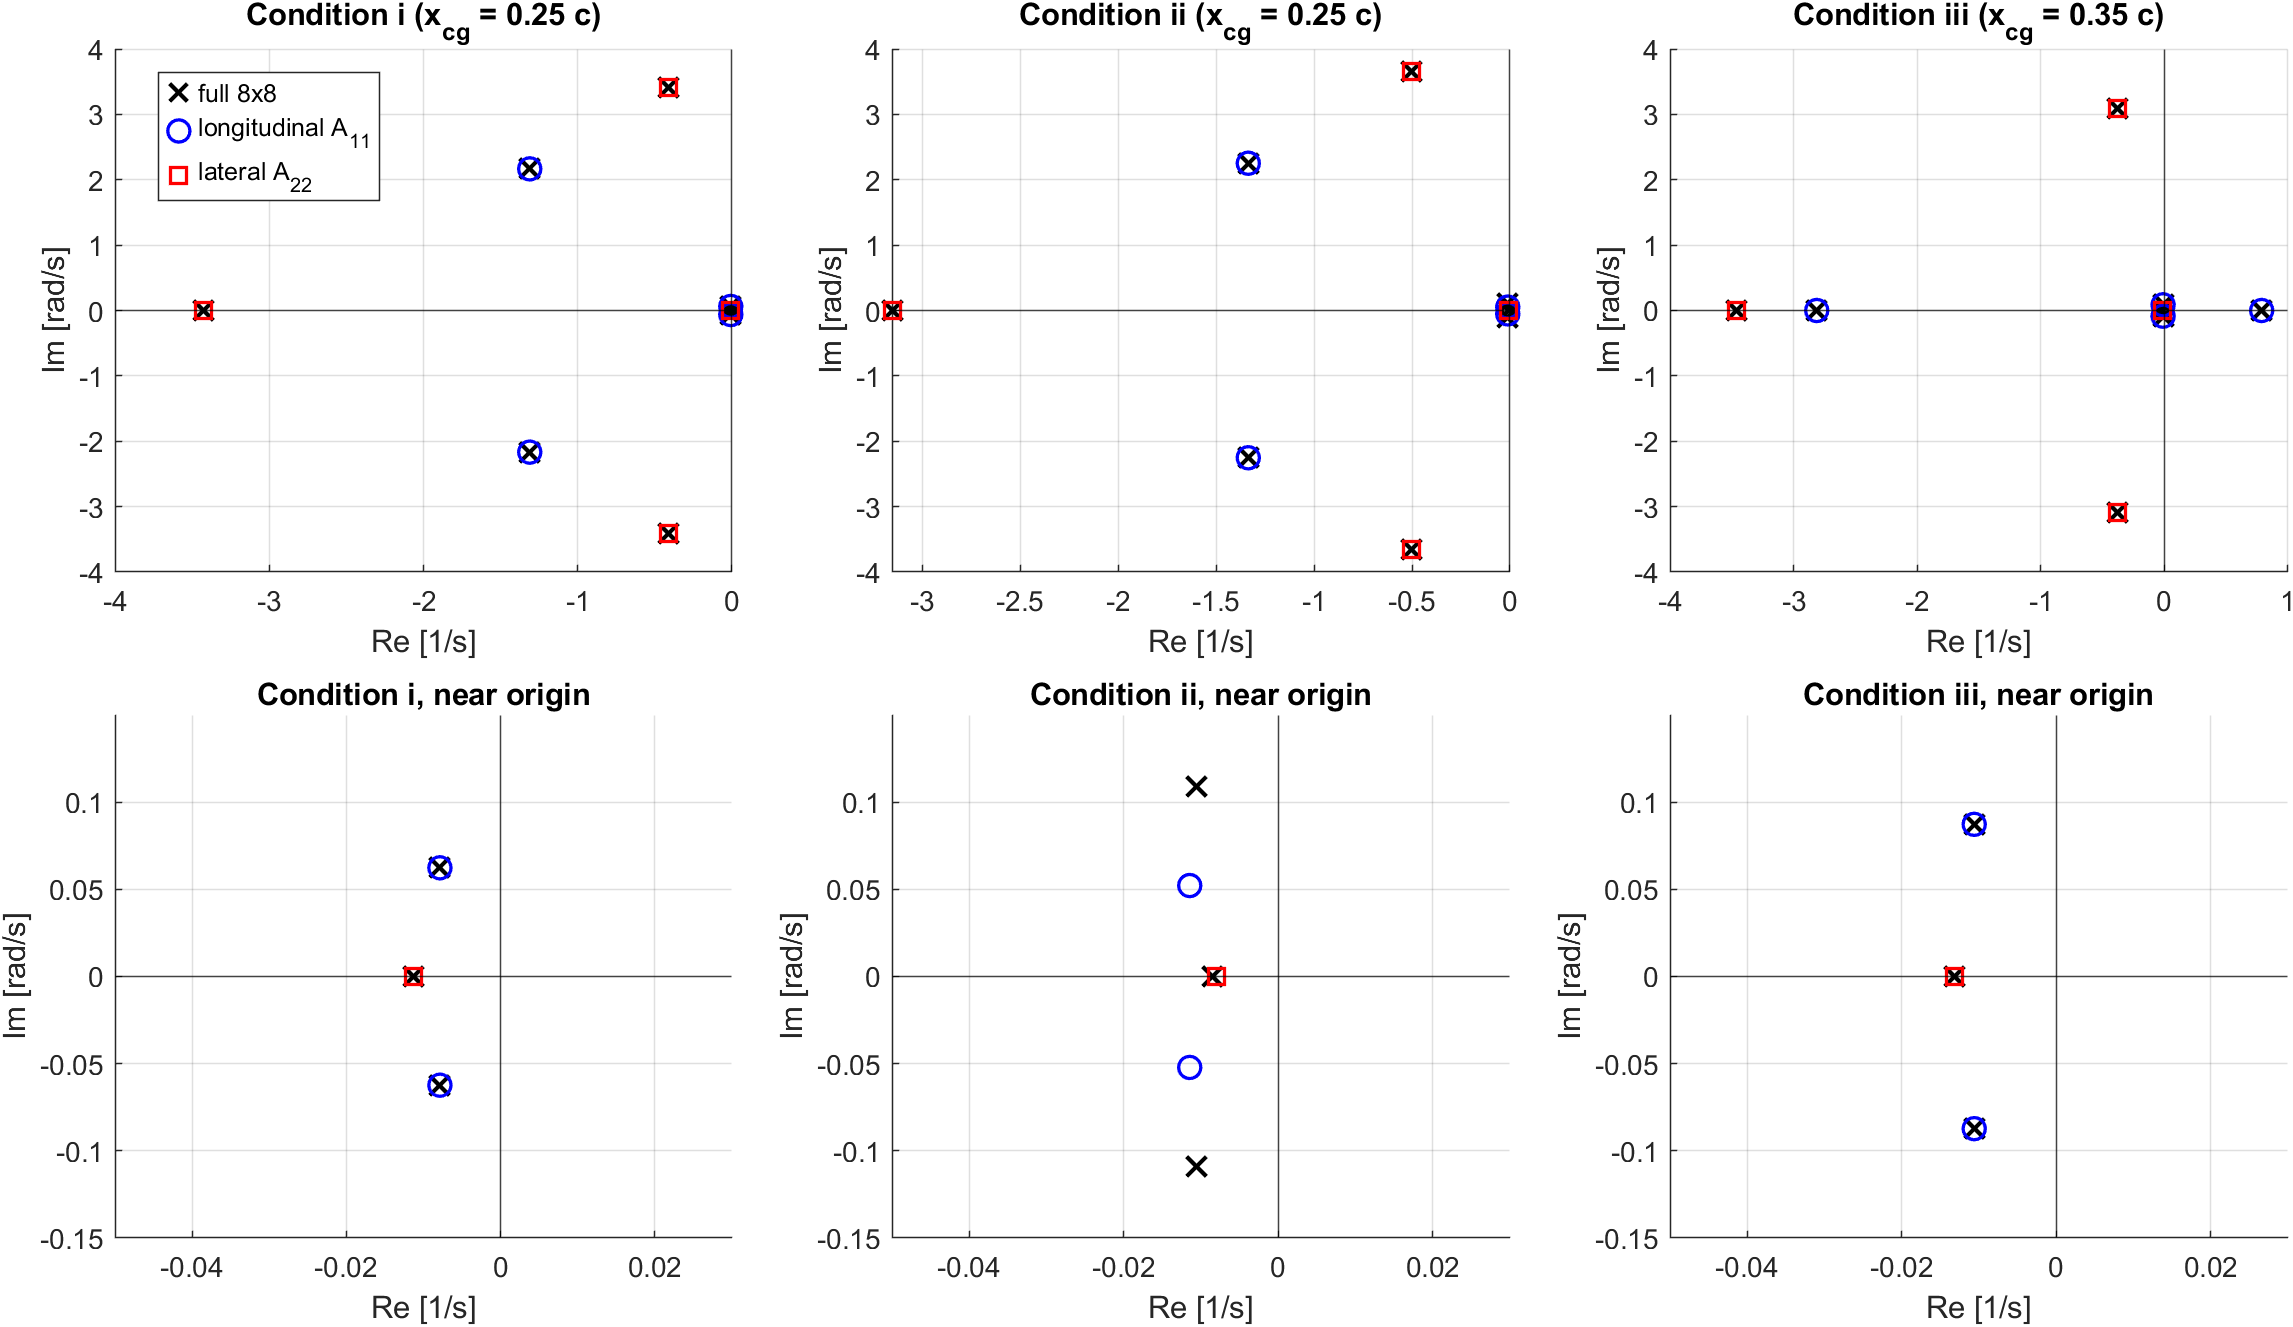
\includegraphics[width=\textwidth]{figures/MT_Eigenvalues.png}
\caption{Tam modelin ve ayrık blokların özdeğerleri (üst) ve başlangıç noktası yakınındaki yavaş modlar (alt).}
\label{fig:eig}
\end{figure}

\subsection{Koşulların karşılaştırılması}
Tablo~\ref{tab:modes} ve Şekil~\ref{fig:eig} sonuçları vermektedir. i koşulunda bütün modlar kararlı ve klasik yapıdadır: iyi sönümlü bir kısa periyot ($\omega_n=2,53$~rad/s, $\zeta=0,52$), 101~s periyotlu, az sönümlü bir fugoid, hızlı bir yuvarlanma modu ($\tau=0,29$~s), kararlı bir spiral mod ($t_{1/2}=61$~s) ve az sönümlü bir Hollanda yuvarlanması ($\omega_n=3,44$~rad/s, $\zeta=0,12$).

Ağırlık merkezinin $0,35\bar c$'ye kaydırılması (iii koşulu) $M_\alpha$'nın işaretini değiştirir ve kısa periyot eşleniği $+0,787$ ve $-2,813$~s$^{-1}$ köklerine ayrılır. Bir bozuntu 0,88~s'de iki katına çıkar; dolayısıyla LEF sabitken çıplak gövde uçuş kontrol sistemi olmadan uçurulamaz. Azalan statik ve yönsel kararlılık fugoid periyodunu 72~s'ye uzatır ve Hollanda yuvarlanması frekansını 3,12~rad/s'ye düşürür; yuvarlanma ve spiral modları az değişir.

Dönüşte (ii koşulu) hızlı modlar i koşuluna göre az değişir; Hollanda yuvarlanmasının sönümü 0,14'e çıkar, yuvarlanma modu ise $\tau=0,32$~s'ye yavaşlar. En çok değişen yavaş modlardır; bunun nedeni aşağıda açıklanan bağlaşımdır.

Karşılaştırma için, Sınıf IV bir uçağın Kategori B uçuş fazındaki MIL-F-8785C sınırlarına göre~\cite{lec7}, i ve ii koşulları kısa periyot sönümü ($0,30\le\zeta\le2$), fugoid sönümü ($\zeta>0,04$), Hollanda yuvarlanması ($\zeta\ge0,08$, $\zeta\omega_n\ge0,15$, $\omega_n\ge0,4$) ve yuvarlanma zaman sabiti ($\tau\le1,4$~s) için Seviye~1 sınırlarını sağlar ve spiral modları kararlıdır. iii koşulunun $t_2=0,88$~s olan kararsız kısa periyot kökü ise Seviye~3'ün $t_2\ge6$~s şartını bile sağlamaz.

\subsection{Tam ve ayrık modeller}
Düz uçuşta (i ve iii) $A_{12}$ ve $A_{21}$ bağlaşım blokları sıfırdır; tam model ile ayrık blokların modları yaklaşık $10^{-5}$ bağıl farkla örtüşür. Dönüşte ise bağlaşım blokları sıfır değildir: yatış açısı düşey kuvvet dengesine girer ($\partial\dot V_T/\partial\phi=-0,673$, $\partial\dot V_T/\partial\beta=8,56$) ve trim açısal hızları yunuslama ile sapmayı birbirine bağlar. Hızlı modlar neredeyse etkilenmez (Tablo~\ref{tab:modesdec}); ancak frekansları birbirine yakın olan fugoid ve spiral modları etkileşir. Tam modelde fugoid periyodu 120~s'den 57~s'ye, sönümü 0,21'den 0,10'a düşer; spiral zaman sabiti ise 126~s'den 117~s'ye değişir. Özvektörler bu karışımı doğrular: boyuna pay fugoid eşleniği için 0,68, spiral kök için 0,53'tür. Fiziksel olarak, dönüşte yatış açısındaki bir değişim kaldırmanın düşey bileşenini değiştirir ve hız değişimiyle birlikte bir tırmanma veya alçalma başlatır; ortaya çıkan hız ve yunuslama değişimleri de dönüşü değiştirir. Bu nedenle ayrık bloklar dönüş uçuşundaki yavaş dinamiği yanlış temsil eder; orada tam model kullanılmalıdır.

\section{Sonuçlar}
\begin{enumerate}
\item Ödev~1'de kurulan ve Ödev~2'de trimlenen model, kumandalar sabitken kanatlar düz uçuşta ve $60^\circ$ yatışlı bir tam dönüş boyunca trimi korur: sapmalar $10^{-2}$~m/s ve $10^{-3}$ derecenin altında kalır; dönüş, trim dönüş hızını ve kuramsal dönüş yarıçapını \%0,2 içinde verir.
\item Benzetimlerdeki küçük artık hareketler dinamik modları gösterir: i koşulunda fugoid ve sönen Hollanda yuvarlanması, ii koşulunda bağlaşık fugoid--spiral salınımı.
\item Ağırlık merkezi $0,35\bar c$'deyken uçak yunuslamada statik olarak kararsızdır ($C_{m_\alpha}=+0,156$~rad$^{-1}$, nötr nokta yaklaşık $0,31\bar c$); 8 durumlu modelin kısa periyot modu $t_2=0,88$~s olan kararsız bir köke ayrılır. Doğrusal olmayan modeldeki LEF tarifesi bunu benzetimde de görülen yavaş bir ıraksamaya ($+0,044$~s$^{-1}$) indirir.
\item Öndeki ağırlık merkezinde bütün türevler olağan işaretlerine sahiptir. Veriler Mach sayısına bağlı olmadığından $C_{D_u}$ ve $C_{m_u}$ düz uçuşta sıfırdır; itki ise sıfırdan farklı bir $X_{T_u}$ ekler.
\item Dönüş uçuşunda $A$'nın elemanları aerodinamik türevlerin yanında eylemsizlik ve jiroskopik terimler de içerir ve boyuna ile yanal-yönsel yavaş modlar birbirine bağlanır; orada tam model gereklidir.
\end{enumerate}

\begin{thebibliography}{9}
\bibitem{tp1538} Nguyen, L. T., Ogburn, M. E., Gilbert, W. P., Kibler, K. S., Brown, P. W., ve Deal, P. L., ``Simulator Study of Stall/Post-Stall Characteristics of a Fighter Airplane With Relaxed Longitudinal Static Stability,'' NASA TP-1538, 1979.
\bibitem{slj} Stevens, B. L., Lewis, F. L., ve Johnson, E. N., \emph{Aircraft Control and Simulation: Dynamics, Controls Design, and Autonomous Systems}, 3. baskı, John Wiley \& Sons, Hoboken, NJ, 2016.
\bibitem{lec5} ``Lecture 5 -- Linearization of Equations of Motion,'' UUM 523E ders notları, İstanbul Teknik Üniversitesi, Güz 2026--2027.
\bibitem{lec6} ``Lecture 6 -- Longitudinal and Lateral-Directional Dynamics,'' UUM 523E ders notları, İstanbul Teknik Üniversitesi, Güz 2026--2027.
\bibitem{lec7} ``Lecture 7 -- Flying and Handling Qualities,'' UUM 523E ders notları, İstanbul Teknik Üniversitesi, Güz 2026--2027.
\end{thebibliography}

\end{document}
